% ============================================================================
% Detecting unknown arbuscular mycorrhizal fungi from linked long-read rDNA copies.
% 11 pt article, booktabs/threeparttable tables, embedded bibliography,
% explicit VERIFY/TODO marks (same conventions as the open-world ITS paper).
% Compile: pdflatex main.tex (twice).
%
% Result numbers are macros: numbers_static.tex (typed by hand, TODO) and
% numbers_generated.tex (analysis/make_numbers.py, from the run outputs). Tables 5, 6
% and S3 are generated too. Figure 1 comes from analysis/make_figures.py.
% ============================================================================
\documentclass[11pt]{article}
\usepackage[utf8]{inputenc}
\usepackage[T1]{fontenc}
\usepackage[a4paper,margin=1in]{geometry}
\usepackage{graphicx}
\usepackage{amsmath}
\usepackage{booktabs}
\usepackage{threeparttable}
\usepackage{longtable}
\usepackage{authblk}
\usepackage{xcolor}
\usepackage[protrusion=true,expansion=false]{microtype}
\usepackage{url}
\usepackage{xurl}
\usepackage[hidelinks]{hyperref}
\renewcommand{\ttdefault}{cmtt}

% Line numbers for review copies: uncomment both lines.
% \usepackage{lineno}
% \linenumbers

% Draft marks. \draftmarksfalse typesets a clean copy: every VERIFY and TODO
% disappears without touching the body text.
\newif\ifdraftmarks
\draftmarkstrue
\definecolor{todoblue}{rgb}{0.0,0.25,0.75}
\ifdraftmarks
  \newcommand{\verify}[1]{\textcolor{red}{[VERIFY: #1]}}
  \newcommand{\todo}[1]{\textcolor{todoblue}{[TODO: #1]}}
\else
  \newcommand{\verify}[1]{}
  \newcommand{\todo}[1]{}
\fi

\renewcommand{\topfraction}{0.9}
\renewcommand{\bottomfraction}{0.7}
\renewcommand{\textfraction}{0.1}
\renewcommand{\floatpagefraction}{0.75}

\newcommand{\spn}[1]{\emph{#1}}   % species names

% ============================================================================
% Static result numbers: curation and compatible-set counts, typed by hand from the
% Stage 3 logs (culture reference v4, fingerprint 181938d695f3df40). Benchmark and M4 numbers are NOT here: they are written by
% analysis/make_numbers.py into numbers_generated.tex.
% ============================================================================
% Culture reference (freeze_ref.py; culture_ref/v4, fingerprint 181938d695f3df40)
\newcommand{\NCopiesIn}{904}
\newcommand{\NCopiesRetained}{903}
\newcommand{\NCultures}{151}
\newcommand{\NSpecies}{37}
\newcommand{\NDivergent}{51}
\newcommand{\NShort}{43}
\newcommand{\NShortCultures}{24}
\newcommand{\NSameLen}{8}
\newcommand{\RefFingerprint}{\texttt{181938d695f3df40}}

% Crosswalk: the counts on culture reference v4 are generated (make_numbers.py, crosswalk section).
% The general UNITE release was run on an earlier version of the reference (same 903 windows);
% per-copy calls do not depend on culture labels, so the count holds for v4.
\newcommand{\SHAssignedGen}{383}
\newcommand{\SHAssignedGenPct}{42\%}

% Compatible sets (arm_sets.py on v4)
\newcommand{\VTDelta}{0.6}
\newcommand{\VTResolved}{16}
\newcommand{\VTResolvedZero}{19}
\newcommand{\SHMerged}{35}
\newcommand{\SHResolved}{32}
\newcommand{\LSUResolved}{27}



% Stefani et al. (2025), New Phytologist: PacBio rDNA of 148 cultures of 44 species; glomalin,
% H+-ATPase and RPB1 for 143 cultures of 39 species (abstract and Methods)
\newcommand{\StefaniCultures}{148}
\newcommand{\StefaniSpecies}{44}
\newcommand{\StefaniPCCultures}{143}
\newcommand{\StefaniPCSpecies}{39}
      % hand-typed curation, crosswalk and calibration counts
% GENERATED by analysis/make_numbers.py; do not edit. See numbers_static.tex for the rest.
% culture-bridge benchmark (compare_its_rule.py)
\newcommand{\KnownN}{755}
\newcommand{\HeldN}{803}
\newcommand{\SingletonN}{48}
\newcommand{\KnownKeptBase}{748}
\newcommand{\ExactBase}{603}
\newcommand{\FKBase}{215}
\newcommand{\FKBasePct}{26.8\%}
\newcommand{\SingletonFKBase}{3}
\newcommand{\KnownKeptClade}{751}
\newcommand{\ExactClade}{701}
\newcommand{\FKClade}{71}
\newcommand{\FKCladePct}{8.8\%}
\newcommand{\SingletonFKClade}{0}
\newcommand{\KnownKeptITS}{745}
\newcommand{\ExactITS}{697}
\newcommand{\FKITS}{18}
\newcommand{\FKITSPct}{2.2\%}
\newcommand{\SingletonFKITS}{0}
\newcommand{\ExactITSPct}{92.3\%}
\newcommand{\FKITSSpeciesMacro}{1.4\%}
\newcommand{\FKITSCultureMacro}{1.9\%}
% divergent-class copies of species held by another culture (culture holdout, placement + N6)
\newcommand{\DivN}{42}
\newcommand{\DivRecognised}{35}
\newcommand{\DivKnown}{3}
\newcommand{\DivNovel}{4}
\newcommand{\ShortRecCulture}{36}
\newcommand{\ShortRecSpecies}{29}
% exact species from one arm alone, known-species copies, culture holdout
\newcommand{\ArmExactVT}{370}
\newcommand{\ArmExactVTPct}{49\%}
\newcommand{\ArmExactSH}{343}
\newcommand{\ArmExactSHPct}{45\%}
\newcommand{\ArmExactLSU}{351}
\newcommand{\ArmExactLSUPct}{46\%}
\newcommand{\ReconExact}{607}
\newcommand{\ReconExactPct}{80\%}
\newcommand{\TreeDemoted}{4}
% the ITS rule on known-species copies (culture holdout, placement + N6)
\newcommand{\ITSDemotedKnown}{6}
\newcommand{\ITSDemotedKnownPct}{0.8\%}
\newcommand{\ITSDemotedText}{4 from \emph{G.\ chinense} 4036\_906B, 1 from \emph{G.\ rosea} CU131\_1018E, 1 from \emph{M.\ litorea} 5274}
\newcommand{\LitoreaITS}{12.6\%}
\newcommand{\ITSThrTypical}{6.0\%}
\newcommand{\ITSThrTypicalFolds}{139 of 148}
\newcommand{\FKITSVarAes}{9}
\newcommand{\FKITSChiRug}{9}
% held-out copies moving from "novel species, genus known" to "novel lineage" (placement)
\newcommand{\GenusLoss}{146}
% empty when the M4 species run is complete
\newcommand{\MfourComplete}{}
\newcommand{\MfourFolds}{34}
\newcommand{\MfourAllFolds}{37}
\newcommand{\RugFull}{4}
\newcommand{\RugFullITS}{4}
\newcommand{\RugRemoved}{75}
\newcommand{\RugRemovedITS}{62}
\newcommand{\RugN}{75}
\newcommand{\RugRescued}{13}
\newcommand{\ChiFull}{28}
\newcommand{\ChiFullITS}{5}
\newcommand{\ChiRemoved}{28}
\newcommand{\ChiRemovedITS}{5}
\newcommand{\ChiN}{35}
\newcommand{\ChiRescued}{23}
\newcommand{\MfourHeldN}{673}
\newcommand{\MfourFKvOne}{78}
\newcommand{\MfourFKvTwo}{53}
\newcommand{\MfourFKvOnePct}{11.6\%}
\newcommand{\MfourFKvTwoPct}{7.9\%}
\newcommand{\MfourControlFKvOne}{19}
\newcommand{\MfourControlFKvTwo}{9}
\newcommand{\MfourControlPct}{2.8\%}
\newcommand{\MfourControlTwoPct}{1.3\%}
\newcommand{\MfourFKvOneSpeciesMacro}{20.6\%}
\newcommand{\MfourFKvTwoSpeciesMacro}{11.7\%}
\newcommand{\MfourGenusN}{673}
\newcommand{\MfourGenusCalled}{326}
\newcommand{\MfourGenusCompatible}{326}
\newcommand{\MfourGenusWrong}{0}
\newcommand{\MfourAbsentTarget}{Ambispora callosa}
\newcommand{\MfourAbsentFK}{20/20}
\newcommand{\MfourAbsentFKvTwo}{0/20}
% the largest groups of remaining false-known calls (first-outcome folds, v2)
\newcommand{\MfourRemaining}{\emph{D.\ aestuarii} called \emph{D.\ varaderana} (20), \emph{R.\ irregularis} called \emph{{[}R.{]}\ vesiculiferum} (18), \emph{D.\ arenaria} called \emph{D.\ jakucsiae} (4), \emph{D.\ jakucsiae} called \emph{D.\ arenaria} (4), \emph{G.\ macrocarpum} called \emph{G.\ rugosae} (4), \emph{D.\ varaderana} called \emph{D.\ aestuarii} (3)}
\newcommand{\MfourRemainingPairs}{6}
\newcommand{\MfourNovelSpecies}{272}
\newcommand{\MfourNovelLineage}{347}
\newcommand{\MfourKnownCalls}{53}
\newcommand{\MfourOtherCalls}{1}
% demotions to "novel species, genus known" by reason code (first-outcome folds, v2)
\newcommand{\MfourNOne}{18}
% demotions to "novel species, genus known" by reason code (first-outcome folds, v2)
\newcommand{\MfourNTwo}{195}
% demotions to "novel species, genus known" by reason code (first-outcome folds, v2)
\newcommand{\MfourNThree}{34}
% demotions to "novel species, genus known" by reason code (first-outcome folds, v2)
\newcommand{\MfourNSix}{25}
\newcommand{\MfourNOnePct}{2.7\%}
% M4 genus folds (genus withheld from the cultures and from V18)
\newcommand{\GenusFolds}{15}
\newcommand{\GenusMainN}{852}
\newcommand{\GenusHeldN}{803}
\newcommand{\GenusFKvOne}{0}
\newcommand{\GenusFKvTwo}{0}
\newcommand{\GenusNovelLineage}{734}
\newcommand{\GenusWrongN}{69}
\newcommand{\GenusWrongPct}{8.6\%}
\newcommand{\GenusWrongText}{\spn{Rhizophagus} called \spn{Sclerocystis} (69)}
\newcommand{\GenusControlWrong}{0}
\newcommand{\GenusDivN}{51}
\newcommand{\GenusDivRecognised}{0}
\newcommand{\GenusDivWrong}{40}
\newcommand{\GenusBoundary}{5}
% species complexes (species_groups.py, distance rule on the frozen reference)
\newcommand{\NComplexes}{4}
\newcommand{\NComplexSpecies}{9}
\newcommand{\ITSSpread}{6.0\%}
\newcommand{\LSUSpread}{3.0\%}
\newcommand{\SSUSpread}{0.8\%}
\newcommand{\NearMissPair}{\emph{D.\ celata} with \emph{D.\ eburnea}}
\newcommand{\NearMissMarker}{LSU}
\newcommand{\NearMissPoints}{0.4}
\newcommand{\NearMissNext}{0.7}
\newcommand{\ComplexCopies}{255}
\newcommand{\ComplexCopiesPct}{29.9\%}
\newcommand{\FKInsideVOne}{54}
\newcommand{\FKOutsideVOne}{24}
\newcommand{\FKOutsideVOnePct}{3.6\%}
\newcommand{\FKInsideVTwo}{53}
\newcommand{\FKOutsideVTwo}{0}
\newcommand{\FKOutsideVTwoPct}{0.0\%}
\newcommand{\FKInsideCtlOne}{9}
\newcommand{\FKOutsideCtlOne}{10}
\newcommand{\FKOutsideCtlOnePct}{1.5\%}
\newcommand{\FKInsideCtlTwo}{9}
\newcommand{\FKOutsideCtlTwo}{0}
\newcommand{\FKOutsideCtlTwoPct}{0.0\%}
% held-out copies whose genus is held by another culture (first-outcome folds)
\newcommand{\GenusRepN}{487}
\newcommand{\GenusRepRight}{326}
\newcommand{\GenusRecallPct}{66.9\%}
\newcommand{\GenusRepLost}{161}
\newcommand{\GenusUnrepN}{186}
% N6 and complexes at the 95.0th percentile
\newcommand{\PctNinetyFiveFK}{37}
\newcommand{\PctNinetyFiveFKPct}{5.5\%}
\newcommand{\PctNinetyFiveOutside}{5}
\newcommand{\PctNinetyFiveComplexes}{3}
\newcommand{\PctNinetyFiveKnownDemoted}{32}
\newcommand{\PctNinetyFiveKnownDemotedPct}{4.2\%}
\newcommand{\PctNinetyFiveSpeciesFK}{9}
\newcommand{\PctNinetyFiveSpeciesFKPct}{1.1\%}
\newcommand{\PctNinetySevenHalfFK}{53}
\newcommand{\PctNinetySevenHalfFKPct}{7.9\%}
\newcommand{\PctNinetySevenHalfOutside}{18}
\newcommand{\PctNinetySevenHalfComplexes}{3}
\newcommand{\PctNinetySevenHalfKnownDemoted}{22}
\newcommand{\PctNinetySevenHalfKnownDemotedPct}{2.9\%}
\newcommand{\PctNinetySevenHalfSpeciesFK}{13}
\newcommand{\PctNinetySevenHalfSpeciesFKPct}{1.6\%}
\newcommand{\PctNinetyNineFK}{53}
\newcommand{\PctNinetyNineFKPct}{7.9\%}
\newcommand{\PctNinetyNineOutside}{0}
\newcommand{\PctNinetyNineComplexes}{4}
\newcommand{\PctNinetyNineKnownDemoted}{6}
\newcommand{\PctNinetyNineKnownDemotedPct}{0.8\%}
\newcommand{\PctNinetyNineSpeciesFK}{18}
\newcommand{\PctNinetyNineSpeciesFKPct}{2.2\%}
% R. irregularis copies called [R.] vesiculiferum (first-outcome folds, with N6)
\newcommand{\RirrVesN}{18}
% GenBank deposit (organism and culture fields)
\newcommand{\DepositLabels}{148}
\newcommand{\DepositNames}{41}
\newcommand{\DepositSpecies}{36}
\newcommand{\DepositGenusOnly}{5}
\newcommand{\RefNames}{41}
\newcommand{\RefGenusOnly}{4}
% crosswalk counts (crosswalk.py report on the final reference v4; analysis/crosswalk_replay.py)
\newcommand{\XwCultures}{151}
\newcommand{\XwNamedCultures}{138}
\newcommand{\XwNamedSpecies}{37}
\newcommand{\VTAssigned}{895}
\newcommand{\SHAssignedFull}{592}
\newcommand{\SHAssignedFullPct}{66\%}
\newcommand{\LSUAssigned}{750}
\newcommand{\VTSpeciesMulti}{3}
\newcommand{\VTSpeciesN}{37}
\newcommand{\VTUnitsMulti}{8}
\newcommand{\VTUnitsN}{30}
\newcommand{\SHSpeciesMulti}{22}
\newcommand{\SHSpeciesN}{34}
\newcommand{\SHUnitsMulti}{0}
\newcommand{\SHUnitsN}{70}
\newcommand{\LSUSpeciesMulti}{3}
\newcommand{\LSUSpeciesN}{36}
\newcommand{\LSUUnitsMulti}{3}
\newcommand{\LSUUnitsN}{36}
\newcommand{\SHSplitByVT}{0}
\newcommand{\SHSplitByVTN}{77}
\newcommand{\SHSplitByLSU}{1}
\newcommand{\SHSplitByLSUN}{73}
\newcommand{\LSUSplitByVT}{4}
\newcommand{\LSUSplitByVTN}{40}
\newcommand{\VTSplitBySH}{24}
\newcommand{\VTSplitBySHN}{30}
\newcommand{\SHSplitCultures}{74}
\newcommand{\SHSplitDenom}{107}
\newcommand{\SHSplitMax}{6}
\newcommand{\LSUOwnSpecies}{105}
\newcommand{\LSUOwnDenom}{135}
\newcommand{\LSUOwnPct}{78\%}
\newcommand{\LSUCongener}{24}
\newcommand{\LSUNoCall}{6}
\newcommand{\LSUGenusRight}{all}
% divergent copies (crosswalk.py section 6)
\newcommand{\DivSHMedian}{99.8\%}
\newcommand{\MainSHMedian}{99.1\%}
\newcommand{\SameLenN}{8}
\newcommand{\SameLenCultures}{5}
% SHs reached by divergent-class copies; of them, reached by no / one main-type copy
\newcommand{\DivSHs}{14}
\newcommand{\ParalogSH}{11}
\newcommand{\DivSHOneMain}{3}
\newcommand{\ParalogPlaceholder}{4}
   % written by analysis/make_numbers.py from the run outputs
% GENERATED by analysis/lgdb_numbers.py from the LongGloDB test outputs; do not edit.
% LongGloDB test set (lgdb_test.py, 06_scores)
\newcommand{\LgTestASVs}{280}
\newcommand{\LgTestCultures}{52}
\newcommand{\LgKnownN}{164}
\newcommand{\LgKnownCultures}{22}
\newcommand{\LgNovelN}{102}
\newcommand{\LgNovelSpN}{59}
\newcommand{\LgNovelLinN}{43}
\newcommand{\LgNovelCultures}{26}
\newcommand{\LgNovelSpecies}{19}
\newcommand{\LgGenusOnlyN}{14}
% condition B folds; species V18 does not hold by label
\newcommand{\LgFolds}{19}
\newcommand{\LgAbsentByLabel}{0}
% M4 parity before scoring
\newcommand{\LgParityCopies}{850}
\newcommand{\LgParityFolds}{37}
\newcommand{\LgParityA}{903}
% VT arm: test ASVs with a hit passing the frozen coverage
\newcommand{\LgVTAnchor}{33}
\newcommand{\LgVTAnchorSpanned}{280}
\newcommand{\LgSHAnchor}{209}
\newcommand{\LgNSixThreshold}{6.0\%}
\newcommand{\LgFK}{4}
\newcommand{\LgFKPct}{3.9\%}
\newcommand{\LgFKSpMacro}{5.3\%}
\newcommand{\LgFKCuMacro}{3.8\%}
\newcommand{\LgFKNovelSp}{4}
\newcommand{\LgFKNovelLin}{0}
% same, without N6
\newcommand{\LgFKvOne}{4}
\newcommand{\LgFKCase}{\spn{Gigaspora gigantea} KS302 called \spn{G.\ rosea}}
\newcommand{\LgFKITSRange}{0.5--2.0\%}
% V18 species clade of the false-known ASVs with V18 intact (condition A)
\newcommand{\LgFKLSUCladeA}{\spn{Gigaspora gigantea}}
% novel ASVs with the same status and placement in A and B
\newcommand{\LgABSame}{102}
\newcommand{\LgLSUUnmatchedB}{97}
\newcommand{\LgFKA}{4}
\newcommand{\LgSecFK}{5}
\newcommand{\LgSecFKPct}{4.9\%}
\newcommand{\LgSecFKSpMacro}{10.5\%}
\newcommand{\LgSecFKCuMacro}{7.7\%}
% secondary VT: ASVs whose VT state changes (condition A)
\newcommand{\LgSecVTChanged}{251}
\newcommand{\LgSecStatusChanged}{66}
% novel species in held genera, primary B
\newcommand{\LgGenusRight}{6}
\newcommand{\LgGenusWrong}{0}
\newcommand{\LgNovelSpAsLineage}{44}
\newcommand{\LgBoundary}{9}
\newcommand{\LgLinGenusGiven}{0}
\newcommand{\LgLinAsLineage}{43}
% secondary VT, B
\newcommand{\LgSecGenusRight}{29}
\newcommand{\LgSecGenusWrong}{0}
\newcommand{\LgSecLinGenusGiven}{18}
\newcommand{\LgSecWrongGenusDetail}{the 18 ASVs of \spn{Racocetra gregaria} were given \spn{Cetraspora}}
\newcommand{\LgSecWrongGenusVT}{VTX00041}
% known species, condition A, primary, with N6
\newcommand{\LgKept}{136}
\newcommand{\LgKeptPct}{82.9\%}
\newcommand{\LgKeptvOne}{151}
\newcommand{\LgKeptvOnePct}{92.1\%}
\newcommand{\LgNSixDemoted}{15}
\newcommand{\LgWrongSp}{8}
\newcommand{\LgWrongSpDetail}{\spn{Funneliformis coronatus} MR101 called \spn{F.\ mosseae}}
\newcommand{\LgWrongSpITSRange}{0.0--0.6\%}
\newcommand{\LgSecKept}{139}
\newcommand{\LgSecKeptvOne}{154}
\newcommand{\LgNSixDemotedITSRange}{6.1--9.6\%}
% D1 calls among test ASVs, A primary
\newcommand{\LgDOne}{1}
% A. leptoticha MX982A: full-ITS distance to the nearest reference culture
\newcommand{\LgLeptoMXITS}{7.8--9.6\%}
% LongGloDB composition (longglodb_overlap.py)
\newcommand{\LgTotal}{1{,}122}
\newcommand{\LgStefani}{810}
\newcommand{\LgStefaniIdentical}{784}
% known-species ASVs identical in ITS to a reference copy of their species
\newcommand{\LgIdentN}{43}
\newcommand{\LgIdentKept}{40}
\newcommand{\LgNonIdentN}{121}
\newcommand{\LgNonIdentKept}{96}
\newcommand{\LgNonIdentKeptPct}{79.3\%}
% G. rosea test cultures with ASVs within 0.5% (ITS) of the group-A types
\newcommand{\LgRoseaCultures}{BR155B, FL105 and KS885}
\newcommand{\LgRoseaMaxITS}{0.25\%}
\newcommand{\LgCodeShared}{4}
\newcommand{\LgCodeConflicts}{3}
% the lock (predictions.predictions.tsv)
\newcommand{\LgLockedN}{4}
\newcommand{\LgFKOutsideLocked}{0}
\newcommand{\LgSecFKOutsideLocked}{1}
\newcommand{\LgPredInsideOwn}{139}
\newcommand{\LgPredInsideOwnKept}{135}
\newcommand{\LgPredOutsideOwn}{25}
\newcommand{\LgPredOutsideOwnNotKept}{24}
\newcommand{\LgWrongSpPredicted}{8}
\newcommand{\LgSecExtraFKDetail}{\spn{Septoglomus constrictum} KS890 called \spn{S.\ africanum} / \spn{S.\ turnauae}}
\newcommand{\LgSecExtraFKITS}{1.1\%}
        % written by analysis/lgdb_numbers.py from the LongGloDB test outputs
% GENERATED by analysis/complex_pcgenes.py from the Stefani et al. (2025) protein-coding records; do not edit.
\newcommand{\PcRecords}{419}
\newcommand{\PcConflicts}{6}
\newcommand{\PcConflictDetail}{FS16\_2427A (\spn{Diversispora epigaea} in the reference, \spn{Septoglomus} sp. in GenBank); FS\_9\_2328B (\spn{Septoglomus} sp. in the reference, \spn{[Rhizoglomus] vesiculiferum} in GenBank); Gwalkeri\_IVT132A (\spn{[Rhizoglomus] vesiculiferum} in the reference, \spn{Diversispora epigaea} in GenBank)}
\newcommand{\PcConflictNearest}{0.0--0.9\%}
\newcommand{\PcBaseline}{42 of 44 on glomalin; 43 of 45 on RPB1; 43 of 45 on H$^+$-ATPase}
\newcommand{\PcBaselinePct}{95--96\%}
\newcommand{\PcComplexPairsN}{4}
\newcommand{\PcComplexPairsAll}{6}
\newcommand{\PcComplexAboveN}{2}
\newcommand{\PcComplexAbove}{\spn{D.\ aestuarii} and \spn{D.\ varaderana} on RPB1 (1.24\% against 1.1\%); \spn{R.\ irregularis} and \spn{[R.]\ vesiculiferum} on glomalin (1.32\% against 1.0\%)}
\newcommand{\PcComplexClean}{0}
\newcommand{\PcComplexCleanText}{none}
\newcommand{\PcComplexComparisons}{12}
\newcommand{\PcMissing}{\spn{G.\ chinense} / \spn{G.\ macrocarpum}; \spn{G.\ macrocarpum} / \spn{G.\ rugosae}}
     % written by analysis/complex_pcgenes.py from the protein-coding records

\title{\textbf{Detecting unknown arbuscular mycorrhizal fungi from linked long-read rDNA copies}}
\author[1]{Aaron O'Brien\thanks{Corresponding author: aaron.obrien@unab.cl}}
\affil[1]{Centro de Biotecnolog\'ia de Sistemas, Universidad Andr\'es Bello, Santiago, Chile}
\date{}

\begin{document}
\maketitle

\begin{abstract}
\noindent
1.~Arbuscular mycorrhizal fungi (AMF) are named in environmental DNA by three
systems that rarely agree: MaarjAM virtual taxa (VT) from the SSU, UNITE species
hypotheses (SH) from the ITS, and clades on LSU reference trees. We asked how
reliably a call combining the three names known species and flags unknown ones.

\noindent
2.~We cut \NCopiesRetained{} long-read rDNA copies from \NCultures{} cultures of
\NSpecies{} named species into the barcode windows each database was built on,
linked the three systems on the same molecules, and combined compatible units into
one call, with every link fitted on training cultures only. We withheld species from
the cultures and the LSU reference, and tested \LgTestCultures{} cultures from other
collections (LongGloDB) against locked predictions.

\noindent
3.~The systems mostly nest, SHs inside LSU species inside VTs, but VTs resolve at
most \VTResolvedZero{} of \NSpecies{} species, and the main-type copies of
\SHSplitCultures{} of \SHSplitDenom{} cultures span 2--\SHSplitMax{} SHs.
Copies with a shortened 5.8S mimic new lineages. Main-type copies of species held by another
culture kept a compatible known call in \KnownKeptITS{} of \KnownN{} cases. For
withheld species, \MfourFKvOnePct{} of copies were called known, and
\MfourFKvTwoPct{} after a culture-ITS distance rule; with the species left in the
LSU reference these fell to \MfourControlPct{} and \MfourControlTwoPct{}, so much of
the novelty signal came from the external reference. The genus of a withheld species
was kept for only \GenusRecallPct{} of copies whose genus another culture holds. All \FKInsideVTwo{} remaining
errors lie inside \NComplexes{} species complexes (\NComplexSpecies{} species) whose
members overlap on all three markers; one exists only at the 99th percentile
used to define them. With MaarjAM and UNITE intact, this may understate errors for species without a VT
by up to \MfourNOnePct{} of copies. On LongGloDB,
\LgFK{} of \LgNovelN{} ASVs of species absent from the reference were called known,
all as predicted; there the ITS rule prevented no error and cost
\LgNSixDemoted{} of \LgKnownN{} known-species calls.

\noindent
4.~Novelty can be called reliably only above the resolution of the markers, and
species they cannot separate should be reported as groups. Linked long-read copies
also bridge the three naming systems empirically.

\vspace{0.6em}
\noindent
\textbf{Keywords.} arbuscular mycorrhizal fungi; Glomeromycota; rDNA
intragenomic variation; MaarjAM; UNITE; novelty detection; phylogenetic
placement; long-read metabarcoding.
\end{abstract}

% ============================================================================
\section{Introduction}
% ============================================================================
AMF surveys name what they find in three incompatible ways, so results from
different markers cannot be pooled. SSU studies report MaarjAM virtual taxa
\cite{opik2010maarjam,opik2014virtual}; ITS studies report UNITE species hypotheses
\cite{koljalg2013unified,nilsson2019unite}; LSU studies place reads on curated
reference trees \cite{kruger2012phylogenetic,delavaux2021lsu,delavaux2022lsu,delavaux2024lsu}.
No agreed table maps one system onto another, and global occurrence databases keep the
datasets apart \cite{vetrovsky2023globalamfungi}. The names in the three databases were
assigned independently, many reference sequences are unidentified environmental clones,
and the taxonomy itself keeps moving: the family Glomeraceae alone has recently been
divided into several families \cite{dasilva2024families}.

AMF genomes make the mapping harder. Their rDNA copies are not homogenised:
copies within one individual differ \cite{pawlowska2004organization}, a single
\spn{Rhizophagus irregularis} genome carries only ten or eleven complete 45S units
that differ in sequence and are not arranged in tandem \cite{maeda2018rdna}, and
copies within a culture can differ by several percent in ITS
\cite{vankuren2013rdna,stefani2025rdna}. One genome can therefore look like several
taxa in ITS, and a divergent copy can look like an unknown lineage. Any claim of AMF
novelty has to rule these out first. Novelty calls have been calibrated for fungal ITS
generally \cite{obrien2026flag}, but not for the AMF case, where three naming systems
and intragenomic variation interact.

Long reads spanning the SSU, ITS and LSU link all three markers on one molecule.
Amplicons of about 2.5~kb were introduced to consolidate the three barcoding regions into
one dataset \cite{kolarikova2021pacbio}, and a large collection of such copies from
identified cultures now exists \cite{stefani2025rdna}. It lets each copy be named by
all three systems at once, and each culture serves as ground truth for its own copies. We
use it to ask four questions:
\begin{enumerate}
\item How do VTs, SHs and LSU clades map onto each other and onto cultured species?
\item Which divergent copy classes exist, and how does each mislead naming?
\item Can compatible calls from the three markers be combined into one reliable name?
\item How often is a species the reference does not know called a known species,
and how much does the answer depend on what the external databases contain?
\end{enumerate}
This work comes from amfsplit, a long-read AMF metabarcoding tool built on ITSxRust v0.3.0
\cite{obrien2026itsxrust}. We report the part that bridges the naming systems and tests novelty
calls (Stage~3). Cutting reads into the legacy windows (Stage~1) is described only as far as the
deposited copies need; its performance on environmental libraries, and the copy-aware abundance
model (Stage~2), will be reported with the tool.

% ============================================================================
\section{Methods}
% ============================================================================
Every step below reads a frozen, versioned culture reference, and every quantity
learned from cultures is refitted inside each validation fold.

\subsection{Regions and legacy windows}
\label{sec:stage1}
\paragraph{Anchors and ITS regions.} ITSxRust anchors each read with one nhmmer pass
(HMMER~3 \cite{eddy2011hmmer}, ITSx fungal profile \cite{bengtsson2013itsx}) and delimits
the SSU flank, ITS1, 5.8S, ITS2, full ITS and LSU flank. We use tolerant anchoring
thresholds (E-value $\le10^{-3}$, anchor score $\ge15$): anchoring only delimits regions.

\paragraph{Legacy windows.} A panel of seven windows (Table~\ref{tab:stage1}) is cut at the
original primer sites, so each window covers the region its legacy database was built on.
The panel uses the primers of the SSU virtual taxa (NS31, AM1, AML2
\cite{simon1992specific,helgason1998ploughing,lee2008improved,opik2010maarjam}), the SSU V4
primers WANDA and AMV4.5NF/AMDGR \cite{dumbrell2011distinct,sato2005}, the LSU primers
LROR \cite{bunyard1994morchella,delavaux2021lsu} and FLR2 \cite{trouvelot1999visualization}, the D2 primers
FLR3 and FLR4 \cite{gollotte2004diversity}, and the outer pair AML1 and LSUmBr
\cite{lee2008improved,kruger2009dna} of the long amplicon \cite{kolarikova2021pacbio}, LSUmBr as the
degenerate consensus of its five variants \cite{schlaeppi2016profiling}.
Primers are located with an IUPAC-aware infix alignment (edlib \cite{sosic2017edlib}) that
tolerates edits up to 15\% of the primer length; windows are primer-trimmed, and coordinates are
1-based, inclusive and in rRNA-sense orientation. Every primer sequence was checked against published
sources (\texttt{analysis/primer\_check.tsv}).
A primer is searched only in the part of the read where it can lie (SSU primers before the ITS, LSU
primers after it, plus 50~nt). A window is \emph{open} when a primer site lies beyond the end of
the copy, and \emph{missing} when the primer is absent although the copy covers its expected position.
Copies were also screened for repeats (concatemers) with the screen of amfsplit version~0.3.1, which
will be described with the tool.

\subsection{Data and regions}
We used the \NCopiesIn{} rDNA copies deposited by Stefani et al.\
\cite{stefani2025rdna} (GenBank PX207096--PX207274 and PX214440--PX215164). Their study reports
PacBio rDNA for \StefaniCultures{} cultures of \StefaniSpecies{} species, and the three protein-coding genes
for \StefaniPCCultures{} cultures of \StefaniPCSpecies{} phylogenetic species; only the rDNA copies are used here. The
deposit carries \DepositLabels{} culture labels and, in its organism fields, \DepositNames{} names
(\DepositSpecies{} species and \DepositGenusOnly{} named only to genus), the same names as their culture tables
(Tables S2 and S3 there). Their \StefaniPCSpecies{} protein-coding species are phylogenetic species, which
split \spn{Septoglomus} sp.\ into three; the \StefaniSpecies{} rDNA species are not itemised, and we use
the deposit's names. Three labels hold two lineages each
(mixed cultures), which we count as separate cultures, hence \NCultures{}. After the name edits
(Table~\ref{tab:edits}) the reference holds \RefNames{} names: \NSpecies{} named species and
\RefGenusOnly{} named only to genus. Stage~1
cut each copy into the SSU flank, ITS1, 5.8S, ITS2, full ITS, the LSU LROR--FLR2
window and the D2 window; all \NCopiesIn{} copies were anchored. Sequences were
compared with edlib \cite{sosic2017edlib} using infix edit distance as a percentage
of the shorter sequence.

\subsection{Culture reference}
A culture is an organism name plus a culture label. \texttt{freeze\_ref.py} builds
the reference from the Stage~1 tables and an edits file. Every edit states first
what the data must look like (organism, label, copy count, VT, copy class, 5.8S
length), and a failed expectation stops the build before anything is written. Each
version records input and output hashes and a fingerprint. The edits leading to
version~4 (fingerprint \RefFingerprint) are listed in Table~\ref{tab:edits}.

Copy classes follow the 5.8S. Stage~1 flagged copies whose 5.8S is more than 3\%
from the culture medoid. We split the flagged copies into \emph{short-5.8S} copies,
at least 3~bp shorter than the culture's main type, and \emph{same-length} copies.
Where the medoid fell inside the short-5.8S group the flags came out inverted, and
the classes were swapped (Table~\ref{tab:edits}).

\subsection{External references and assignment arms}
The VT arm used the MaarjAM gDAT snapshot of July 2020 \cite{opik2010maarjam}, the
SH arm UNITE release 10.0 of 19 February 2025 \cite{nilsson2019unite,unite2025release},
and the LSU arm the Delavaux V18 database of May 2025 \cite{delavaux2021lsu,delavaux2022lsu,delavaux2024lsu}
(repository commit \texttt{f4a0014}). Searches used BLAST+ \cite{camacho2009blast}
with the settings in Table~\ref{tab:arms}. Many V18 records carry terminal N
padding, so coverage does not count reference Ns; without that correction 95 of
460 records fail the coverage test even against themselves. Hits to any accession
of the culture reference were dropped, so no copy could take a name from itself or
a culture-mate. A culture's label on an arm is the modal label of its main-type copies (ties go to
the higher median identity). A copy's calls depend only on its window, the database and the dropped
accessions, not on culture names. The crosswalk was run before the last two \spn{Septoglomus} edits
(Table~\ref{tab:edits}), so its culture-level report was replayed on the final labels with the stored
per-copy calls (\texttt{crosswalk\_replay.py}), after checking every stored call against per-unit
evidence captured on the final reference: on all three arms and all \NCopiesRetained{} copies the
call's identity equals that of the highest-scoring hit passing the threshold, and the best unit is
present at that identity.

\begin{table}[htbp]\centering
\begin{threeparttable}
\caption{The three assignment arms. Each copy is searched with BLAST+ against one
external reference per arm; all arms require e-value $\le10^{-50}$.}
\label{tab:arms}
\small
\begin{tabular}{lllp{0.30\linewidth}rr}
\toprule
Arm & Query region & Task & Reference & Identity & Coverage\\
\midrule
VT  & SSU flank  & megablast & MaarjAM (gDAT, July 2020; 3{,}081 seq., 384 VT) & $\ge97\%$   & $\ge95\%$\\
SH  & full ITS   & blastn & UNITE 10.0, UNITE+INSD (16{,}800 Glomeromycota seq., 7{,}563 SH) & $\ge98.5\%$ & $\ge90\%$\\
LSU & LROR--FLR2 & blastn & Delavaux V18 (460 AMF records, 234 species labels) & $\ge97\%$ & $\ge90\%$\\
\bottomrule
\end{tabular}
\begin{tablenotes}\footnotesize
\item Coverage is of the shorter sequence, with reference Ns not counted. Hits to
any accession of the culture reference are dropped. The SH arm was also run
against the UNITE general release (2{,}048 Glomeromycota representatives).
\end{tablenotes}
\end{threeparttable}
\end{table}


\subsection{Compatible unit sets}
Each copy receives a set of units instead of a single best hit. The anchor is the
copy's best hit by bit score, and the set holds every unit within $\delta$ identity
points of the anchor that also passes the identity threshold. Units that split one
culture's main-type copies at $\delta=0$ are merged when the closest copies across
the split are within 1\% in the SSU flank; that limit keeps the two lineages of a
mixed culture from being merged. $\delta$ is the smallest margin at which the
main-type copies of at least 99\% of cultures share a unit. On the VT arm it is
also at least the 95th percentile of within-culture SSU spread. SH and LSU carry no
such floor, because their within-genome spread is wide and uneven (95th percentile:
ITS 8.6\%, LROR--FLR2 3.9\%), and the merged units carry that variation instead.

\subsection{LSU phylogenetic placement}
The V18 references were realigned with MAFFT \cite{katoh2013mafft}, and branch
lengths and GTR+$\Gamma_4$ parameters were fitted on the published topology with
RAxML-NG \cite{kozlov2019raxmlng}. Queries were added with
\texttt{--addfragments --keeplength} and placed with EPA-ng
\cite{barbera2019epang}. The compatible edges of a query carry at least 95\% of
its likelihood weight. Edges inside a maximal clade bearing a single V18 species
label are collapsed into one unit (the \emph{species-clade} rule). Where a species label is not
monophyletic on the backbone, its separate components stay separate units, and edges that carry
several species labels stay individual units.

\subsection{Reconciliation}
A unit is linked to the species and genera of the training cultures whose culture
set holds it. In each arm a copy is \emph{matched} when its units belong to
training cultures, \emph{unmatched} when it has a call but no training culture
holds the unit, and \emph{silent} when it has no call. Genera are intersected over
matched arms and species over the matched arms that name species. The call is a
species, a species group, a genus, discordant or unplaced.

\subsection{Novelty decision tree}
The tree tests the cheapest explanation first.
\begin{enumerate}
\item \textbf{Artifact (A1).} Against the nearest main-type copy of another
culture, the SSU differs by at least 1\% and by at least half the ITS difference.
\item \textbf{Divergent class,} read from the copy itself. D1: the 5.8S is at
least 3~bp shorter and at least 3\% different from comparators of the baseline
length. D2: the best-hit VT or SH is reached, in at least two other cultures,
only by short-5.8S copies.
\item \textbf{Boundary (B1).} No VT call, but the best VT lies within one point of
the 97\% threshold.
\item \textbf{Novelty.} A species call is demoted to ``novel species, genus known''
when the VT or LSU arm is unmatched (N1, N2), or when the full-ITS distance to the
nearest copy of any training culture exceeds the 99th percentile of within-species
distance between training cultures (N6). No matched arm gives ``novel lineage''.
\end{enumerate}

\subsection{Species complexes}\label{sec:complexes}
Some pairs of named species cannot be told apart from the markers. We define this from the
reference alone. For each marker (full ITS, LROR--FLR2, SSU flank) the within-species spread is the
99th percentile of the distance from a main-type copy to the nearest main-type copy of another culture
of the same species (ITS \ITSSpread{}, LSU \LSUSpread{}, SSU \SSUSpread{}). Two species are
\emph{inseparable} when, on every marker, their nearest copies lie no further apart than that spread:
a copy of one then falls inside the spread of the other. Connected pairs form a complex, and a
complex is reported as a unit wherever a species call is made (\texttt{species\_groups.py}). The rule
uses no test result and adds no threshold beyond the 99th percentile already used for the ITS rule,
computed the same way (Python's exclusive quantile method). To see how much the conclusions depend on
that choice, the ITS rule and the complexes were also set together at the 95th and the 97.5th
percentile: the rule was re-applied to the stored decision-tree rows with each fold's limit refitted
on its training cultures (\texttt{percentile\_sensitivity.py}).

\subsection{Validation design}
Every culture-derived quantity is fitted on training cultures only within each fold:
merged units, $\delta$, unit-to-species links, D1 comparators, D2 support, the
nearest-copy pools and the N6 threshold. \emph{Culture holdout} has 148 folds, each
removing one physical culture label together with all lineages sharing it.
\emph{Species holdout} has 50 folds, one per named species with all its cultures
removed plus one per unnamed culture. A \emph{false known} is a known species or
species-group call for a copy whose species has no training culture.

In these benchmarks the MaarjAM, UNITE and V18 databases stay fixed. The external
holdout (M4) removes each target species from V18 as well: V18 is realigned, the
model refitted and all copies re-placed. MaarjAM and UNITE are not edited in
any fold, so a withheld species keeps whatever virtual taxon and species hypothesis it has there;
this matters because an unmatched virtual taxon demotes a call (N1) and an unmatched SH does not.
Protocol~v2 adds N6 and changes nothing else; \spn{G.\ chinense} and \spn{G.\ rugosae} informed that
rule and are reported as development folds. The \emph{first-outcome folds} are all other species folds:
\MfourFolds{} in which the target's V18 records were removed, and one (\spn{\MfourAbsentTarget})
whose species V18 does not hold by label, which is reported apart. The same protocol also has \GenusFolds{} genus folds, in
which every culture of a genus and the genus's V18 records are withheld together. The cohort was used to develop the methods, so all figures
from it are development results; the independent test is described next.

\subsection{Independent cultures}\label{sec:lgdb-methods}
LongGloDB v1 (July 2026) \cite{glodb} holds \LgTotal{} curated SSU--ITS--LSU amplicon sequence variants
(ASVs) from AMF culture collections. \LgStefani{} of them carry the laboratory codes STFP and STFI and
were left out: \LgStefaniIdentical{} of these are identical in full ITS to a copy in our reference,
so they are the Stefani cultures reprocessed. \LgCodeShared{} further cultures share a
culture code with a Stefani label (\LgCodeConflicts{} of them under another species name) and were left
out too (\texttt{longglodb\_overlap.py}). The test set is the remaining \LgTestASVs{} ASVs of
\LgTestCultures{} cultures from three other laboratories: \LgKnownN{} ASVs of \LgKnownCultures{}
cultures of species the reference holds, \LgNovelSpN{} of species it does not hold in genera it does,
\LgNovelLinN{} of genera it does not hold, and \LgGenusOnlyN{} named only to genus. The novel ASVs come
from \LgNovelCultures{} cultures of \LgNovelSpecies{} species.

Before any test sequence was searched, placed or scored, the complex rule
(Section~\ref{sec:complexes}) was applied to the test ASVs, and its predictions were locked by hash
together with a protocol and two amendments that fix the outcomes, conditions and analyses
(\texttt{PROTOCOL\_LGDB.md}). A test ASV can be called a known species wrongly only if it lies within the
within-species spread of that species on all three markers, so any false known outside the predicted
set contradicts the result of Section~\ref{sec:errorcomplexes}. The frozen code of protocol~v2 was used
unchanged. All \NCultures{} reference cultures train and every test culture is excluded, so no test
sequence enters merges, margins, unit links, comparators or the N6 threshold. Test sequences were cut by
Stage~1 like the deposited copies, and their VT and SH evidence was computed with the same filtering
against the same releases. In condition~A the test windows are placed on the intact V18; in
condition~B each of the \LgFolds{} novel species, all of which V18 holds by label, is removed from V18 in
its own fold, as in M4.

The test amplicons begin about 60~bp inside the NS31--AM1 region, so a test SSU flank rarely covers
95\% of a MaarjAM reference, and the frozen VT arm finds a passing hit for only \LgVTAnchor{} of
\LgTestASVs{} ASVs. The primary analysis applies the arm as it is. A secondary analysis, fixed before the
run, measures VT coverage over the part of each reference the query spans and changes nothing else.

% ============================================================================
\section{Results}
% ============================================================================
\subsection{Legacy windows on the deposited copies}
All \NCopiesIn{} deposited copies were anchored, and every window whose primers lie inside a
copy was recovered (Table~\ref{tab:stage1}). Median lengths are close to the amplicons behind
the legacy databases: 508~bp for NS31--AM1 with primers removed, about 550~bp with them, the
size of the fragment behind MaarjAM virtual taxa. No window crosses an ITSxRust anchor, and no
copy was flagged as a repeat. The 28 copies without an NS31--AM1 window are exactly the
Paraglomerales copies, in which AM1 does not bind. \begin{table}[htbp]\centering
\begin{threeparttable}
\caption{Legacy barcode windows cut from the 904 deposited rDNA copies (amfsplit v0.3.1,
primer-trimmed windows, up to 15\% of each primer's length in edits).}
\label{tab:stage1}
\footnotesize\setlength{\tabcolsep}{3pt}
\begin{tabular}{llrrrr}
\toprule
Window & Target & Usable & Missing & Open & Median (bp)\\
\midrule
SSU NS31--AM1        & MaarjAM VT       & 876 & 28 (3$'$) & 0  & 508\\
SSU NS31--AML2       & SSU studies      & 904 & 0         & 0  & 522\\
SSU WANDA--AML2      & SSU V4           & 903 & 1 (5$'$)  & 0  & 500\\
SSU AMV4.5NF--AMDGR  & SSU V4, short    & 904 & 0         & 0  & 216\\
LSU LROR--FLR2       & Delavaux LSU     & 904 & 0         & 0  & 735\\
LSU FLR3--FLR4 (D2)  & LSU D2           & 904 & 0         & 26 (3$'$) & 330\\
AML1--LSUmBr         & full amplicon    & 0   & 904 (both) & 0 & --\\
\bottomrule
\end{tabular}
\begin{tablenotes}\footnotesize
\item Usable = complete plus open-ended windows; missing = primer absent although the copy covers its position; open = site beyond the copy end. The 28 missing NS31--AM1 windows are all
the Paraglomerales copies, in which AM1 does not bind; the one missing WANDA window is
the copy dropped from the reference (PX215117.1). The 26 open D2 windows are copies that end
before the FLR4 site. The outer amplicon primers are absent because the deposited copies are
trimmed inside them. No window crosses an ITSxRust anchor, and none of the 904 copies is
flagged as a concatemer.
\end{tablenotes}
\end{threeparttable}
\end{table}


\subsection{Reference curation}
Names are used as deposited, with genus synonyms (\spn{Rhizoglomus} and \spn{Rhizophagus}) treated
as equal where genera are compared; the reorganisation of the Glomerales
\cite{dasilva2024families} postdates most deposits, and a name that is outdated in a database
is not an error of the marker. The name check went against the expected relabelling. T3\_IVT34A and CC4\_4A\_IVT7A
are \spn{R.\ irregularis} by ITS and LSU (for example ITS2 3.3\% against 6.4\% for
T3), yet their SSU falls in VTX00113, so VTX00113 holds both \spn{R.\ irregularis}
and \spn{R.\ vesiculiferum}. In SD5\_IVT32 the corrected main type matches V18
\spn{R.\ proliferus} at 98.5--99.9\%, while its short-5.8S copies are 91.8\% from
anything in V18. Two \spn{Septoglomus} cultures, SO43BL and Blasz\_17\_2277A, carry
the same two lineages with the majority reversed; the lineages differ like species
(ITS1 11--12\%, 5.8S 5.7\%, LSU 1.6\%). Version~4 holds \NCopiesRetained{} copies
in \NCultures{} cultures of \NSpecies{} named species, with \NDivergent{}
divergent-class copies (\NShort{} short-5.8S, \NSameLen{} same-length).
\begin{table}[htbp]\centering
\begin{threeparttable}
\caption{Culture reference edits from the deposited copies to v4.}
\label{tab:edits}
\small
\begin{tabular}{p{0.28\linewidth}p{0.20\linewidth}p{0.42\linewidth}}
\toprule
Item & Edit & Evidence\\
\midrule
PX215117.1 (\emph{G.\ rosea}) & dropped & SSU and ITS diverge at the same rate (4--6\% and 5.6--7.6\%): error or pseudogene\\
BR105\_2435A & second lineage split off as \emph{Paraglomus} sp. & three VTX00281 copies 28--33\% from the culture's \emph{P.\ brasilianum} copies in ITS\\
4375\_IVT88A, ON205A & labels merged & one culture filed under two organism names\\
T3\_IVT34A, CC4\_4A\_IVT7A & kept as \emph{R.\ irregularis} & name check: ITS2 3.3\% vs 6.4\% (T3); LSU nearest \emph{R.\ irregularis}\\
SD5\_IVT32, 212939\_IVT38A & main and divergent classes swapped & medoid fell in the short-5.8S group\\
SO43BL, Blasz\_17\_2277A & mixed cultures split; SO43BL named \emph{S.\ africanum} & reciprocal lineages; ITS and LSU agree on \emph{S.\ africanum}\\
\bottomrule
\end{tabular}
\end{threeparttable}
\end{table}


\subsection{The three systems nest}
The SSU flank assigns \VTAssigned{} of \NCopiesRetained{} copies to a VT. Counting
cultures by their modal label, \VTSpeciesMulti{} of \VTSpeciesN{} named species span more than one VT and
\VTUnitsMulti{} of \VTUnitsN{} VTs hold more than one species; VTX00199 alone holds four \spn{Glomus}
species. The LSU nearest reference gives a culture's own species for \LSUOwnSpecies{} of
\LSUOwnDenom{} named cultures whose species V18 holds (\LSUOwnPct{}; \LSUCongener{} get a congener and
\LSUNoCall{} no call) and the right genus for \LSUGenusRight{} that get a call, but V18 holds two records for nearly every species (460 records under 234 species labels:
215 labels with two records, five with three or four, 14 with one), and 45 of the 220 labels with
two or more records hold two records under 97\% apart, and in leave-one-out on V18 itself only 72\% of records
return their own species. The full UNITE+INSD set assigns \SHAssignedFull{} copies
(\SHAssignedFullPct{}) against \SHAssignedGen{} (\SHAssignedGenPct{}) for the general
release, which keeps one representative per SH. An SH is finer than a genome: the
main-type copies of \SHSplitCultures{} of \SHSplitDenom{} cultures with two or more
SH calls fall in two to \SHSplitMax{} SHs. Counting each culture by its modal SH, \SHUnitsMulti{} of \SHUnitsN{} SHs hold two named
species and VT splits \SHSplitByVT{} of \SHSplitByVTN{}
SHs; once SHs are merged into per-genome groups, one group is shared by \spn{G.\ macrocarpum} and
\spn{G.\ rugosae}. \SHSplitByLSU{} of \SHSplitByLSUN{} SHs is split by LSU (\spn{D.\ varaderana} / \spn{D.\ bareai}) and \LSUSplitByVT{} of \LSUSplitByVTN{} LSU
units are split by VT. So SH mostly sits inside LSU species, which mostly sit inside VT.

\subsection{Divergent copies and paralog units}
The two divergent classes behave differently on every marker (Table~\ref{tab:divergent}).
Short-5.8S copies are well represented in public data, consistent with the heterogeneous
non-tandem units of a single genome \cite{maeda2018rdna}: their median best SH hit
(\DivSHMedian{}) is closer than the main type's (\MainSHMedian{}). Divergent copies reach \DivSHs{} SHs;
\ParalogSH{} of them no main-type copy reaches (paralog SHs, \ParalogPlaceholder{} under placeholder names),
and \DivSHOneMain{} take one main-type copy each (Table~\ref{tab:paralog}). \spn{S.\ viscosum}'s short copies are the
only culture copies that reach VTX00409, about two points clear of VTX00063.
In \spn{Gigaspora rosea}, four cultures carry the same three or four rDNA types,
identical across cultures and up to 6.2\% apart in LSU, each in its own SH named
\spn{G.\ rosea}. These types are not confined to one isolate held in several collections: in LongGloDB
(Section~\ref{sec:lgdb}), INVAM cultures under other accession codes (\LgRoseaCultures{}; FL105 is INVAM's
reference culture for the species) carry ASVs within \LgRoseaMaxITS{} of them in full ITS.
\begin{table}[htbp]\centering
\begin{threeparttable}
\caption{The two divergent copy classes mislead each marker differently.}
\label{tab:divergent}
\small
\begin{tabular}{p{0.50\linewidth}p{0.18\linewidth}p{0.18\linewidth}}
\toprule
 & Short 5.8S & Same length\\
\midrule
Copies (cultures) & 43 (24) & 8 (5)\\
VT: same as the culture's main type / other / no call & 35 / 7 / 1 & 8 / 0 / 0\\
LSU: same species / another species / no call & 5 / 1 / 31 & 2 / 5 / 1\\
LSU best-hit identity, median (main type 98.9\%) & 94.9\% & 97.2\%\\
SH: same / other SH / no call & 0 / 28 / 7 & 0 / 4 / 1\\
SH best-hit identity, median (main type 99.1\%) & 99.8\% & 98.6\%\\
\bottomrule
\end{tabular}
\begin{tablenotes}\footnotesize
\item Each divergent copy against the modal unit of its culture's main-type copies (crosswalk.py,
culture reference v4). Copies in cultures without a main-type unit on a marker are left out of that
marker's row (short 5.8S: VT 0, LSU 6, SH 8;
same length: VT 0, LSU 0, SH 3).
\end{tablenotes}
\end{threeparttable}
\end{table}

\begin{table}[htbp]\centering
\begin{threeparttable}
\caption{Paralog units: SHs and a VT reached by divergent-class copies and by at most one main-type copy.}
\label{tab:paralog}
\footnotesize\setlength{\tabcolsep}{4pt}
\begin{tabular}{p{0.15\linewidth}p{0.20\linewidth}p{0.34\linewidth}p{0.06\linewidth}p{0.13\linewidth}}
\toprule
Unit & Name of the best hit & Divergent copies & Main & Identity\\
\midrule
SH1337353.10FU & \emph{Rhizophagus irregularis} & \emph{R.\ irregularis} 10 (7 cultures) & 1 & 100.0\%\\
SH1364117.10FU & Glomeromycota sp. & \emph{{[}R.{]}\ vesiculiferum} 7 (2 cultures) & 0 & 98.5--99.8\%\\
SH1081549.10FU & \emph{Rhizophagus} sp. & \emph{R.\ prolifer} 4 (1 culture) & 0 & 99.3--99.8\%\\
SH1081557.10FU & \emph{Rhizoglomus intraradices} & \emph{R.\ intraradices} 4 (3 cultures) & 0 & 100.0\%\\
SH1076762.10FU & \emph{Gigaspora margarita} & \emph{G.\ rosea} 2 (1 culture) & 1 & 99.8\%\\
SH1337340.10FU & \emph{Rhizophagus} sp. & \emph{Rhizophagus} sp. 1; \emph{R.\ irregularis} 1 (2 cultures) & 0 & 100.0\%\\
SH1337458.10FU & \emph{Rhizophagus irregularis} & \emph{R.\ silesianus} 2 (1 culture) & 0 & 100.0\%\\
SH1389224.10FU & Glomeraceae sp. & \emph{S.\ viscosum} 2 (1 culture) & 0 & 100.0\%\\
VTX00409 & environmental (MaarjAM) & \emph{S.\ viscosum} 3 (2 cultures) & 0 & 98.5--99.4\%\\
\bottomrule
\end{tabular}
\begin{tablenotes}\footnotesize
\item \emph{Main}: main-type copies of any culture in the unit. 6 further units take one divergent
copy each (SH1076712, SH1196937, SH1337247, SH1337463, SH1337480, SH1364178). Names are those of the best UNITE record; the VT row is MaarjAM's.
\end{tablenotes}
\end{threeparttable}
\end{table}


\subsection{Compatible sets}
Within-culture SSU spread is small (median 0.07\%, 95th percentile 0.54\%, 99th
0.95\%). Merging two VT pairs, VTX00113+VTX00115 and VTX00125+VTX00222, makes every
culture consistent at $\delta=0$ (Table~\ref{tab:sets}). The VT spread floor
($\delta=\VTDelta$) costs three species of resolution. SH sets, once merged into
per-genome groups, separate \SHResolved{} of \NSpecies{} species against
\VTResolved{} for VT; that figure is an upper bound because the merges are learned
on the same cultures.
\begin{table}[htbp]\centering
\begin{threeparttable}
\caption{Calibrated compatible sets on culture reference v4.}
\label{tab:sets}
\footnotesize\setlength{\tabcolsep}{4pt}
\begin{tabular}{lrrrrp{0.26\linewidth}}
\toprule
Arm & Merged units & $\delta$ & Consistent cultures & One unit & Species resolved\\
\midrule
VT                      & 2  & 0.6 & 138/138 & 74\%  & 16 of 37 (19 at $\delta=0$)\\
SH                      & 35 & 0   & 106/107 & 100\% & 32 of 37\\
LSU (nearest reference) & 5  & 0   & 128/128 & 81\%  & 27 of 37\\
\bottomrule
\end{tabular}
\begin{tablenotes}\footnotesize
\item A culture is consistent when the sets of its main-type copies share a unit.
A named species is resolved when no other named species shares any of its unit
groups. Merged units and species counts are learned and scored on the same
cultures, so they are upper bounds.
\end{tablenotes}
\end{threeparttable}
\end{table}


\subsection{Reconciliation and novelty with the culture bridge held out}
Combining the arms recovers what none reaches alone. Among the \KnownN{} main-type copies of
species held by another culture, with merges and margins fitted on training cultures, the exact
species comes from VT for \ArmExactVT{} (\ArmExactVTPct{}), SH for \ArmExactSH{} (\ArmExactSHPct{}) and
LSU for \ArmExactLSU{} (\ArmExactLSUPct{}), and from the combination for \ReconExact{} (\ReconExactPct{})
before the decision tree; the tree demotes \TreeDemoted{} of them, leaving \ExactBase{}
in Table~\ref{tab:benchmark}. LSU placement raises exact-species calls and cuts false-known calls from \FKBasePct{} to \FKCladePct{},
and the ITS rule cuts them again to \FKITSPct{} (Table~\ref{tab:benchmark},
Figure~\ref{fig:falseknown}a); averaged over species or over cultures the final
rate is \FKITSSpeciesMacro{} and \FKITSCultureMacro{}. The ITS threshold was
\ITSThrTypical{} in \ITSThrTypicalFolds{} culture folds. It demoted \ITSDemotedKnown{} known-species copies
(\ITSDemotedText{}); the \spn{M.\ litorea} copy lies \LitoreaITS{} from the species' other culture.
The \FKITS{} remaining errors are two complexes: \spn{D.\ varaderana} with \spn{D.\ aestuarii}
(\FKITSVarAes{} copies), which are indistinguishable on every marker, and \spn{G.\ chinense} with
\spn{G.\ rugosae} (\FKITSChiRug{} copies), whose ITS spreads overlap. Of the \DivN{} divergent-class copies whose species is held by another culture, \DivRecognised{} were
recognised as divergent class, \DivKnown{} same-length copies were called their own species, and
\DivNovel{} were wrongly called a novel species. Short-5.8S copies were
recognised from their own sequence in \ShortRecCulture{} of \NShort{} cases with
their culture held out and \ShortRecSpecies{} with their species held out.
Placement has a cost: \GenusLoss{} held-out copies lose a genus-level novelty call
and become ``novel lineage''.
\begin{table}[htbp]\centering
\begin{threeparttable}
\caption{Training-only benchmark with the external databases fixed.}
\label{tab:benchmark}
\footnotesize\setlength{\tabcolsep}{4pt}
\begin{tabular}{lrrrr}
\toprule
Configuration & Known kept & Exact species & False known, & False known,\\
 & (of 755) & & all held out (of 803) & single-culture (of 48)\\
\midrule
Nearest-reference LSU & 748 & 603 & 215 (26.8\%) & 3\\
LSU species-clade placement & 751 & 701 & 71 (8.8\%) & 0\\
Placement + ITS rule (N6) & 745 & 697 & 18 (2.2\%) & 0\\
\bottomrule
\end{tabular}
\begin{tablenotes}\footnotesize
\item \emph{Known kept}: main-type copies of species held by another training
culture that receive a known species or species-group call containing the true
species (culture holdout, 148 folds). \emph{False known}: known calls for copies
whose species has no training culture (species holdout, 50 folds). Averaged over
species and over cultures, the final false-known rate is 1.4\% and 1.9\%.
\end{tablenotes}
\end{threeparttable}
\end{table}


\begin{figure}[htbp]\centering
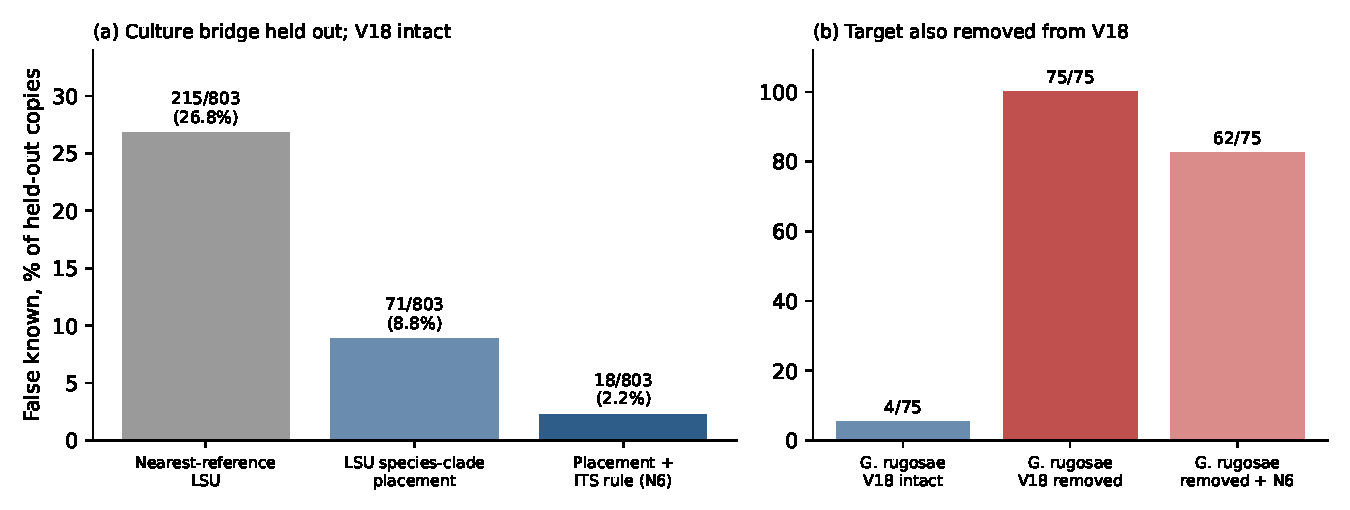
\includegraphics[width=\linewidth]{figures/fig1_falseknown.pdf}
\caption{False-known calls. (a) Species holdout with the external databases fixed,
by configuration. (b) \spn{G.\ rugosae} with the species also removed from V18: the
novelty signal that LSU placement gave came from V18 itself.}
\label{fig:falseknown}
\end{figure}

\subsection{Removing the species from the external LSU reference}\label{sec:external}
With the full V18, \spn{G.\ rugosae} copies fall into V18's own \spn{rugosae} clade,
which no training culture holds, and are flagged as new. With the species removed
they fall into the \spn{chinense} and \spn{macrocarpum} clades and are called known
(Table~\ref{tab:external}, Figure~\ref{fig:falseknown}b). The ITS rule does not use
V18 but rescues only \RugRescued{} of \RugN{} copies, because \spn{G.\ rugosae} ITS lies 1.4--7.5\%
(median 4.7\%) from its relatives, inside ordinary within-species spread.
Pooled over the \MfourFolds{} first-outcome folds, false-known calls among
\MfourHeldN{} copies were \MfourControlFKvOne{} with V18 intact, \MfourFKvOne{} with
the target removed and \MfourFKvTwo{} with the ITS rule (per fold in
Table~\ref{tab:m4folds}); averaged over species the rates are \MfourFKvOneSpeciesMacro{}
and \MfourFKvTwoSpeciesMacro{}. The \MfourFKvTwo{} errors left after the ITS rule fall in \MfourRemainingPairs{} species pairs:
\MfourRemaining. Of the \MfourHeldN{} held-out copies, \MfourNovelSpecies{} were called a novel species in a known
genus (\MfourNTwo{} because the LSU arm was unmatched, \MfourNThree{} because no species was shared
by the arms, \MfourNSix{} by the ITS rule and \MfourNOne{} because the SSU arm was unmatched),
\MfourNovelLineage{} a novel lineage, which carries no genus, \MfourKnownCalls{} a known species or
group, and \MfourOtherCalls{} was flagged as divergent class. The genus was called for
\MfourGenusCalled{} copies and was right for \MfourGenusCompatible{} of them, but that is precision: of the
\GenusRepN{} copies whose genus is held by another culture, the genus was kept for \GenusRepRight{}
(\GenusRecallPct{}), and \GenusRepLost{} were called a novel lineage although their genus was known; the
other \GenusUnrepN{} copies belong to genera with no other culture and were all called a novel lineage. The SSU arm's contribution
to novelty is therefore small (\MfourNOnePct{} of the copies), but it exists: it needs the withheld
species to have a virtual taxon of its own.
The one species V18 does not hold by label, \spn{\MfourAbsentTarget}, was called a known species
for \MfourAbsentFK{} copies without the ITS rule and \MfourAbsentFKvTwo{} with it, because its
ITS lies about 10\% from its closest relative. \MfourComplete{}
\begin{table}[htbp]\centering
\begin{threeparttable}
\caption{Removing the target species from the LSU reference as well.}
\label{tab:external}
\small
\begin{tabular}{llrr}
\toprule
Target & V18 & False known (v1) & With N6 (v2)\\
\midrule
\emph{G.\ chinense}$^{\dagger}$ & full & 28/35 & 5/35\\
\emph{G.\ chinense}$^{\dagger}$ & target removed & 28/35 & 5/35\\
\emph{G.\ rugosae}$^{\dagger}$ & full & 4/75 & 4/75\\
\emph{G.\ rugosae}$^{\dagger}$ & target removed & 75/75 & 62/75\\
\midrule
34 first-outcome folds & full & 19/673 (2.8\%) & 9/673 (1.3\%)\\
34 first-outcome folds & target removed & 78/673 (11.6\%) & 53/673 (7.9\%)\\
\bottomrule
\end{tabular}
\begin{tablenotes}\footnotesize
\item False-known calls among the main-type copies of each fold's target species.
$^{\dagger}$\,Development folds: these two species informed the N6 rule. \emph{Full}: the fold's
copies placed on the intact V18; \emph{target removed}: V18 realigned without the target's records, model
refitted, all copies re-placed. First-outcome folds pool the species whose V18 records were removed; 1 further fold(s) whose species V18 does not hold by label are reported apart.
\end{tablenotes}
\end{threeparttable}
\end{table}


With a whole genus withheld from the cultures and from V18 (\GenusFolds{} folds, \GenusHeldN{} main-type copies
of named species), no copy was called a known species, with or without the ITS rule (\GenusFKvOne{} and
\GenusFKvTwo{}); this is expected, because no training culture shares the genus. \GenusNovelLineage{} copies
were called a novel lineage, the right rank. The other \GenusWrongN{} (\GenusWrongPct{}) were called a novel species in a known genus, and that genus was wrong in every
case: \GenusWrongText{}. With V18 intact, \GenusControlWrong{} copies received a wrong genus. The genus fold shows
at the level of genera what the species folds show at the level of species: a copy whose clade has been removed
is placed on the sister clade, here \spn{Sclerocystis}, and named by the training cultures that hold it. None of
the \GenusDivN{} divergent-class copies was recognised as divergent in these folds (\GenusDivRecognised{}),
because D1 and D2 both need a related culture, and \GenusDivWrong{} of them also received the wrong genus.

\subsection{The remaining errors are species complexes}\label{sec:errorcomplexes}
\NComplexes{} complexes emerge from the distance rule (Table~\ref{tab:complexes}):
\spn{G.\ chinense}, \spn{G.\ macrocarpum} and \spn{G.\ rugosae} (the VTX00199 group);
\spn{D.\ aestuarii} with \spn{D.\ varaderana}; \spn{D.\ arenaria} with \spn{D.\ jakucsiae};
and \spn{R.\ irregularis} with \spn{[R.]\ vesiculiferum}. Together they hold \NComplexSpecies{}
of \NSpecies{} named species and \ComplexCopiesPct{} of the reference copies. One further pair,
\NearMissPair{}, misses the \NearMissMarker{} limit by \NearMissPoints{} points and is not a
complex. The rule depends on the percentile. \spn{D.\ aestuarii} with \spn{D.\ varaderana},
\spn{D.\ arenaria} with \spn{D.\ jakucsiae}, and \spn{G.\ macrocarpum} with \spn{G.\ rugosae} are
complexes at every percentile from the 95th to the 99.5th; \spn{G.\ chinense} joins from the 97.5th,
\spn{R.\ irregularis} with \spn{[R.]\ vesiculiferum} from the 99th, and \spn{F.\ coronatus} with
\spn{F.\ mosseae} at the 99.5th.

The ITS rule uses the same percentile, so a fair test moves both together (Table~\ref{tab:percentile}).
At the 97.5th percentile the rule leaves the same \PctNinetySevenHalfFK{} false-known calls as at the
99th, but the \RirrVesN{} copies of \spn{R.\ irregularis} called \spn{[R.]\ vesiculiferum} now lie outside a
complex. At the 95th the rule is stricter: false known falls to \PctNinetyFiveFK{}
(\PctNinetyFiveFKPct{}), \PctNinetyFiveOutside{} of them outside a complex, all again
\spn{R.\ irregularis} called \spn{[R.]\ vesiculiferum}, at the cost of demoting \PctNinetyFiveKnownDemoted{}
known-species copies in the culture holdout (\PctNinetyFiveKnownDemotedPct{}) instead of
\PctNinetyNineKnownDemoted{}. At every percentile, then, each remaining error is either inside a complex
or this one pair, and whether the pair counts as a complex is the only conclusion that depends on the choice.

Every one of the \FKInsideVTwo{} false-known calls left after the ITS rule in the first-outcome
folds is a call to a member of the species' own complex. Without the ITS rule, \FKInsideVOne{}
of the \MfourFKvOne{} errors are inside a complex and \FKOutsideVOne{} (\FKOutsideVOnePct{}) are
not; with V18 intact the corresponding figures are \FKOutsideCtlOne{} and \FKOutsideCtlTwo{} copies
outside a complex. So the ITS rule removes the errors that the markers could, in principle, have
avoided, and what is left is the limit of the markers themselves. The complexes were derived from
all cultures, including the withheld species, so this shows that the errors are confined to pairs the
reference already shows to be inseparable; it does not show that an undescribed relative of a complex
member would be caught, which it would not, by definition.
\begin{table}[htbp]\centering
\begin{threeparttable}
\caption{Species complexes: pairs of named species whose nearest copies lie within the within-species spread on all three markers.}
\label{tab:complexes}
\footnotesize\setlength{\tabcolsep}{4pt}
\begin{tabular}{llcrrr}
\toprule
Species A & Species B & Complex & ITS & LSU & SSU\\
\midrule
\emph{Diversispora aestuarii} & \emph{Diversispora varaderana} & C2 & 1.1 & 1.09 & 0.0\\
\emph{Diversispora arenaria} & \emph{Diversispora jakucsiae} & C3 & 3.48 & 0.83 & 0.07\\
\emph{Glomus chinense} & \emph{Glomus macrocarpum} & C1 & 5.87 & 2.18 & 0.27\\
\emph{Glomus chinense} & \emph{Glomus rugosae} & C1 & 4.95 & 1.36 & 0.2\\
\emph{Glomus macrocarpum} & \emph{Glomus rugosae} & C1 & 1.38 & 1.36 & 0.07\\
\emph{Rhizophagus irregularis} & \emph{{[}Rhizoglomus{]} vesiculiferum} & C4 & 3.25 & 2.44 & 0.34\\
\bottomrule
\end{tabular}
\begin{tablenotes}\footnotesize
\item Columns give the distance (\%) between the nearest copies of the two species. The limits are the 99th
percentile of the distance between cultures of one species: ITS 6.0\%, LSU 3.0\%, SSU 0.8\%.
\end{tablenotes}
\end{threeparttable}
\end{table}

\begin{table}[htbp]\centering
\begin{threeparttable}
\caption{The ITS rule and the species complexes moved to the same percentile.}
\label{tab:percentile}
\footnotesize\setlength{\tabcolsep}{4pt}
\begin{tabular}{lrrrrrr}
\toprule
Percentile & ITS limit & Complexes & Known demoted & False known, & False known, & Outside\\
 & (median) & (species) & (of 755) & species holdout (of 803) & V18 removed (of 673) & a complex\\
\midrule
95th & 4.4\% & 3 (6) & 32 (4.2\%) & 9 (1.1\%) & 37 (5.5\%) & 5\\
97.5th & 5.0\% & 3 (7) & 22 (2.9\%) & 13 (1.6\%) & 53 (7.9\%) & 18\\
99th & 6.0\% & 4 (9) & 6 (0.8\%) & 18 (2.2\%) & 53 (7.9\%) & 0\\
\bottomrule
\end{tabular}
\begin{tablenotes}\footnotesize
\item The ITS rule is re-applied to the stored decision-tree rows at each percentile, with the limit fitted
on each fold's training cultures, and the complexes are those of the distance rule at the same percentile
(\texttt{percentile\_sensitivity.py}). \emph{Known demoted}: known-species copies the rule demotes in the
culture holdout. \emph{V18 removed}: first-outcome M4 folds. The 99th-percentile row reproduces the reported
results exactly. Every error outside a complex is \emph{R.\ irregularis} called \emph{{[}R.{]}\ vesiculiferum}.
\end{tablenotes}
\end{threeparttable}
\end{table}


\subsection{Cultures from other collections}\label{sec:lgdb}
Before any test result was scored, the \LgParityCopies{} copies of the \LgParityFolds{} M4 species folds
were rescored with the test cultures present and excluded, and every call came back as stored. Adding
the test windows to the V18 alignment left the \LgParityA{} reference alignments and credible unit sets
unchanged.

Among the \LgNovelN{} ASVs of species the reference does not hold, \LgFK{} were called a known species
with the target removed from V18 (\LgFKPct{}; \LgFKSpMacro{} averaged over species, \LgFKCuMacro{} over
cultures; Table~\ref{tab:lgdb}). They are the \LgLockedN{} ASVs the locked prediction placed inside a
reference species, \LgFKCase{}, and \LgFKOutsideLocked{} lie outside the prediction. With V18 intact
their LSU falls in V18's own \LgFKLSUCladeA{} clade, which the reference's \spn{G.\ rosea} cultures also
occupy, and their ITS lies \LgFKITSRange{} from those cultures, so no marker separates the two. None of the
\LgNovelLinN{} ASVs from genera the reference does not hold was called known. Removing the species from
V18 changed no call: \LgABSame{} of \LgNovelN{} novel ASVs had the same status and placement in
conditions A and B, because their LSU fell, in both, in clades no training culture holds. These species
are far from the reference's, and the sister-species case behind the external-removal result
(Section~\ref{sec:external}) occurred once, in KS302, where it was predicted.

Of the \LgKnownN{} ASVs of species the reference holds, \LgKept{} kept their species (\LgKeptPct{}),
against \KnownKeptITS{} of \KnownN{} in the culture holdout. ASVs identical in ITS to a reference copy
kept it in \LgIdentKept{} of \LgIdentN{} cases, the others in \LgNonIdentKept{} of \LgNonIdentN{}
(\LgNonIdentKeptPct{}). The ITS rule demoted \LgNSixDemoted{} of them, whose ITS lies \LgNSixDemotedITSRange{}
from every reference culture, beyond its \LgNSixThreshold{} threshold: without the rule
\LgKeptvOne{} kept their species (\LgKeptvOnePct{}), and it removed no false-known call
(\LgFKvOne{} without it). The \LgWrongSp{} ASVs called another species are \LgWrongSpDetail{},
which the lock had predicted (\LgWrongSpPredicted{} of \LgWrongSp{}): their ITS lies
\LgWrongSpITSRange{} and their SSU 0.0\% from reference \spn{F.\ mosseae} cultures, so the culture is most
likely \spn{F.\ mosseae} under another name. The lock sorted the known species: \LgPredInsideOwnKept{} of
the \LgPredInsideOwn{} ASVs predicted inside their own species kept it, and \LgPredOutsideOwnNotKept{} of
the \LgPredOutsideOwn{} predicted outside did not.

With the frozen VT arm nearly silent, the genus was hard to name: \LgNovelSpAsLineage{} of the
\LgNovelSpN{} ASVs of novel species in genera the reference holds were called a novel lineage and
\LgBoundary{} a VT boundary, and the genus was given for \LgGenusRight{}, all right. With VT coverage
measured over the spanned part, the genus was given for \LgSecGenusRight{}, again all right, but two
errors appeared: \LgSecWrongGenusDetail{}, through a VT the two genera share (\LgSecWrongGenusVT{})
while their LSU was unmatched; and one ASV, \LgSecExtraFKDetail{}, through a shared VT, its ITS
\LgSecExtraFKITS{} from a reference culture. False-known calls then number \LgSecFK{} (\LgSecFKPct{}),
\LgSecFKOutsideLocked{} of them outside the lock.

The test also raised curation questions for the collections. Three culture codes carry different
species in LongGloDB and in the Stefani deposit (MT106, ON205A and BEG9). INVAM's name for both
MT106 and ON205A is \spn{A.\ gerdemannii}, which Stefani et al.\ record and depart from (their Table S2)
and LongGloDB keeps for ON205A. In addition, the LongGloDB
\spn{A.\ leptoticha} MX982A lies \LgLeptoMXITS{} in ITS from the reference's \spn{A.\ leptoticha},
ON205A, which LongGloDB names \spn{A.\ gerdemannii}.
\begin{table}[htbp]\centering
\begin{threeparttable}
\caption{Independent cultures: the frozen rules on 52 LongGloDB cultures from other collections.}
\label{tab:lgdb}
\footnotesize\setlength{\tabcolsep}{4pt}
\begin{tabular}{p{0.10\linewidth}p{0.16\linewidth}p{0.10\linewidth}p{0.07\linewidth}p{0.17\linewidth}p{0.13\linewidth}p{0.11\linewidth}}
\toprule
Analysis & Condition & False known (of 102) & Share & Novel species: genus right / wrong / none (of 59) & Novel genera: genus given (of 43) & Known kept (of 164)\\
\midrule
Primary & A: V18 intact & 4 (4) & 3.9\% & 6 / 0 / 53 & 0 & 136 (151)\\
 & B: target removed & 4 (4) & 3.9\% & 6 / 0 / 53 & 0 & --\\
VT spanned & A: V18 intact & 5 (5) & 4.9\% & 29 / 0 / 30 & 18 & 139 (154)\\
 & B: target removed & 5 (5) & 4.9\% & 29 / 0 / 30 & 18 & --\\
\bottomrule
\end{tabular}
\begin{tablenotes}\footnotesize
\item Protocol v2 (with the ITS rule, N6); in brackets, the same without it. \emph{False known}: ASVs of species the
reference does not hold called a known species or species group. \emph{Novel species}: ASVs of species the reference
does not hold, in genera it holds. \emph{Novel genera}: ASVs of genera it does not hold, so any genus given is wrong.
\emph{Known kept}: ASVs of species the reference holds whose call contains their species; condition A only.
\emph{VT spanned}: the secondary analysis, with VT coverage measured over the part of each MaarjAM reference the
query spans (amendment 2).
\end{tablenotes}
\end{threeparttable}
\end{table}


% ============================================================================
\section{Discussion}
% ============================================================================
Linked copies turn the VT--SH--LSU correspondence from a guess into a measurement,
and show that each naming system fails in its own predictable way.

\paragraph{The bridge is mostly nested, not one-to-one.} SHs mostly sit inside LSU species,
which mostly sit inside VTs. VT counts therefore underestimate species (at best a VT resolves
\VTResolvedZero{} of \NSpecies{}), and SH counts overestimate them, because one
genome spans up to six SHs. Surveys that count SHs as taxa inflate AMF richness, and
part of that inflation is intragenomic. Grouping SHs per genome restores most of the
species signal in our cultures, but the groups are learned from these same cultures
and their transfer to field sequences is untested. The 2.5~kb amplicons were introduced
to consolidate the three regions into one dataset \cite{kolarikova2021pacbio}; what is
missing is a measured correspondence between the names, which the linked copies supply.

\paragraph{Divergent copies are the main source of false taxa.} Intragenomic rDNA variation in
AMF is long established \cite{pawlowska2004organization,vankuren2013rdna}, yet it has been
largely overlooked in ecological and taxonomic work \cite{stefani2025rdna}; what the copies add is
a measurement of how it misleads each marker. Short-5.8S copies
look like novel lineages in LSU and form their own SHs and VTs, several carrying
placeholder names in UNITE. The D1 test recognises most of them from sequence alone,
but recognition falls when the whole species is unknown, since it then lacks a
related culture of the right 5.8S length to compare with. Same-length divergent
copies are more ambiguous: co-dominant types of one genome in \spn{Gigaspora}, second
lineages in \spn{Septoglomus}. They should be flagged, not explained away.

\paragraph{Novelty has a floor set by the markers.} \NComplexes{} complexes, \NComplexSpecies{}
species in all, cannot be separated on SSU, ITS and LSU together: their nearest copies lie inside
each other's within-species spread on every marker. All errors that remain after the ITS rule fall
inside them at the 99th percentile used throughout. The claim holds for every percentile we tried
except for one pair: with the rule and the complexes both at the 95th or 97.5th percentile,
\spn{R.\ irregularis} and \spn{[R.]\ vesiculiferum} are no longer a complex, and the
\spn{R.\ irregularis} copies called \spn{[R.]\ vesiculiferum} are errors outside one
(Table~\ref{tab:percentile}). Whether those two names are separable on rDNA is therefore the open
question, not whether the floor exists. A species call there is honest only as a group, and a novelty call there is not
possible: an undescribed relative inside the spread of a known species is indistinguishable from
that species on these regions. The alternative reading is that some of these names are not separate
lineages, a question for taxonomists; \spn{D.\ aestuarii} and \spn{D.\ varaderana} differ by 0.0\%
in SSU and 1.1\% in LSU. The rule is data-driven and will grow as cultures are added: one further
pair (\NearMissPair{}) misses the \NearMissMarker{} limit by \NearMissPoints{} points.

\paragraph{Novelty depends on what the reference already knows.} With only the
culture bridge held out, LSU placement looks like a strong novelty detector, but
much of that strength comes from the withheld species still being in V18: its clade
holds no culture, so the copy is flagged. Phylogenetic placement was proposed because database matching cannot place sequences from
taxa that are absent from the database \cite{delavaux2021lsu,delavaux2022lsu}. That holds at the
level of clades, but our external-removal folds show its limit at the level of species: with the
species removed, a copy is placed on its nearest named relative and then called by it, and with a genus removed, on
the sister genus (\GenusWrongN{} \spn{Rhizophagus} copies called \spn{Sclerocystis}). An undescribed
species is absent from every reference. Removing it from V18 is therefore closer to the real
situation than leaving it in, but not equal to it: MaarjAM and UNITE were left intact, and many virtual
taxa are built from environmental sequences, so a species that is undescribed yet already sequenced in
the field can still have a virtual taxon of its own. The SSU arm's novelty signal accounts for
\MfourNOne{} of the \MfourHeldN{} copies, so for a species never sequenced the false-known rate may be
higher than reported by up to about \MfourNOnePct{} of the copies. The culture-ITS
rule does not depend on external databases and repairs part of the gap, but not
where ITS itself overlaps. Pooled over the first-outcome folds, false known rose from
\MfourControlPct{} with V18 intact to \MfourFKvOnePct{} with the target removed, and
fell to \MfourFKvTwoPct{} with the ITS rule.

\paragraph{Relation to earlier work on the same cultures.} Stefani et al.\ \cite{stefani2025rdna}
sequenced the copies used here (\StefaniCultures{} cultures of \StefaniSpecies{} species) and compared rDNA
with three protein-coding genes (glomalin, H$^+$-ATPase and RPB1), sequenced for \StefaniPCCultures{}
cultures of \StefaniPCSpecies{} species. They found no barcode gap in any of the
regions, so no single distance threshold identifies AMF, and concluded that rDNA is still the practical
choice because its primers work across all lineages. Our results agree where they overlap: the complexes
are pairs whose nearest copies lie inside each other's spread on every rDNA region. The questions differ.
They ask whether a distance threshold identifies a species within one marker; we ask how the three
naming systems relate and how much novelty can be called once the intragenomic classes are accounted for.
Their protein-coding sequences are public (glomalin PV808915--PV809055, RPB1 PV809056--PV809196,
H$^+$-ATPase PV809197--PV809333) and could settle the complexes: if those genes separate
\spn{D.\ aestuarii} from \spn{D.\ varaderana}, the complex is a limit of rDNA, and if not it is
a question of naming. We compared them (\texttt{complex\_pcgenes.py}; Table~\ref{tab:pcgenes}). At the
thresholds Stefani et al.\ proposed, the three genes separate almost every congeneric pair that rDNA
separates (\PcBaseline{}; \PcBaselinePct{}). Of the \PcComplexPairsAll{} complex pairs, \PcComplexPairsN{}
have protein-coding records for both species. Of these, \PcComplexAboveN{} exceed the threshold on one
gene each (\PcComplexAbove{}), but \PcComplexCleanText{} of the \PcComplexComparisons{} comparisons
exceeds the spread within the species themselves. The complexes are therefore not a limit of rDNA alone: on these
genes, too, their members lie as close as cultures of one species, and whether they are separate species
is a question for taxonomy rather than for the choice of marker. Joining the records through culture names
also showed that the RPB1 and H$^+$-ATPase deposits rotate the species names of three cultures:
\PcConflictDetail{}. Each of these records lies \PcConflictNearest{} from records of its culture's species,
so the sequences are right and the names are not; we left the \PcConflicts{} records out.

\paragraph{Why the rules are not calibrated per species.} A calibrated novelty flag exists for fungal ITS
generally \cite{obrien2026flag}. Here the culture-ITS threshold is itself a calibrated quantile, the
99th percentile of the distance between cultures of one species, and it behaves as set: it demoted \ITSDemotedKnown{} of
\KnownN{} known-species copies (\ITSDemotedKnownPct{}). The 99th percentile was fixed in protocol~v2
before the first-outcome folds were run; the 95th would have cut false-known calls further
(\PctNinetyFiveFKPct{} against \PctNinetyNineFKPct{} with the species removed from V18) at the cost of
demoting \PctNinetyFiveKnownDemotedPct{} of known-species copies instead of \PctNinetyNineKnownDemotedPct{}
(Table~\ref{tab:percentile}), a trade-off a user can set. The other rules, such as the unmatched-arm demotions, are not
calibrated, because the reference holds too few cultures per species to fit a threshold for each,
and because the AMF-specific traps (divergent classes, species complexes) have to be handled before
a calibration can mean anything.

\paragraph{Independent cultures.} On \LgTestCultures{} cultures from three other laboratories, with the
predictions locked before the run, the frozen rules called a species the reference does not hold a known
species only where the complex rule said they would: \spn{G.\ gigantea} KS302, inside \spn{G.\ rosea} on
every marker. The test is easier than ours in one respect and harder in two. Its novel species are far
from the reference's, so it says little about the sister-species case, which occurred once. Its
amplicons start inside the VT region, which leaves the VT arm silent unless coverage is counted over the
part a query spans, and a genus taken from VT alone was then wrong when the true genus was absent from the
reference (\spn{Racocetra} given \spn{Cetraspora}). And its cultures come from other collections, some of
which lie further from ours in ITS than our cultures of one species lie from each other: the ITS rule,
fitted at the 99th percentile on one collection, demoted \LgNSixDemoted{} of \LgKnownN{} known-species
ASVs and prevented no false known. Its threshold should be fitted on more than one collection before the
rule is used on field data.

\paragraph{Implications for surveys.} Name at the level the markers can support:
report VT sets, SH groups per genome and LSU species clades, with species groups
where the markers cannot decide. Screen for the short-5.8S class before counting
taxa, and treat paralog SHs and VTs, such as SH1337353 and VTX00409, as known
genomes. Rest novelty claims on evidence that does not come from the database that
defines ``known'', and read names against a taxonomy that is stated, because outdated names
in a database look like marker errors \cite{dasilva2024families}. Replication across independent
libraries is planned for environmental data.

\subsection{Limitations}
Apart from the LongGloDB test, all results come from one collection of cultured species, and the
cohort was used to develop the methods, so they are development estimates. The LongGloDB test rests on
\LgNovelCultures{} novel cultures, covers distant novelty, and used amplicons on which the frozen VT arm
is silent. The 99th percentile behind the ITS rule
and the complexes was chosen after seeing in-sample distances (Table~\ref{tab:percentile} shows the
effect of other choices), and the complexes are derived from all cultures, including the withheld species. Culture names are treated as
truth, though some are doubtful: \spn{M.\ litorea} 5274, some \spn{G.\ rosea} cultures,
and \spn{Septoglomus} sp.\ C4 and 5070\_5024A, whose LSU matches
\spn{Microviscospora peruviscosa}. MaarjAM and UNITE stay intact in every
benchmark; the external holdout removes species from the LSU reference only. About a quarter of V18's
multi-record species labels (51 in the placement audit) do not form exclusive clades on its backbone. Independent-library replication on environmental data and the Stage~2
abundance model are outstanding.

% ============================================================================
\section{Conclusions}
% ============================================================================
A novelty call for an AMF sequence is only as good as the external references are complete, and
it cannot be made below the resolution of the markers: with the target species removed from the
LSU reference, a share of false known calls remains, and every one of them lies in a species
complex that SSU, ITS and LSU cannot separate. On cultures from other collections, the only species
wrongly called known was the one the complex rule predicted. Linked long-read copies give an empirical bridge
between the three naming systems and show where each one misleads. Divergent copies must be
recognised before taxa are counted, and species that the markers cannot separate, which
protein-coding genes do not separate either, should be reported as groups.

\section*{Data and code availability}
Sequences are GenBank PX207096--PX207274 and PX214440--PX215164. The culture reference
(version~4, \RefFingerprint), the edits files and their manifests, the Stage~3
scripts and the validation packages (training-only bridge, LSU placement, external
holdout with protocols v1 and v2) will be deposited with the paper, as will the LongGloDB test package
(protocol, amendments, locked predictions, runner and score tables); LongGloDB v1 is available from
GloDB \cite{glodb}.
\todo{repository URL and archive DOI} External references: MaarjAM gDAT snapshot
(sha256 \texttt{2b2c57e664e76347\ldots}), UNITE 10.0 of 19 February 2025
\cite{unite2025release} (UNITE+INSD sha256 \texttt{abe98f43e16c179f\ldots}) and
Delavaux V18 AMF-only (sha256 \texttt{e6794cbbe166735a\ldots}).

\section*{Funding}
This work was supported by the Corporaci\'on de Fomento de la Producci\'on (CORFO) through the Programa
Tecnol\'ogico de Transformaci\'on Productiva ante el Cambio Clim\'atico, Agrosimbiosis Program (grant number
23PTECCC-247149).

\section*{Author contributions}
Aaron O'Brien conceived the study, developed the software, carried out the analyses and wrote the
manuscript.

\section*{Acknowledgements}
We thank the maintainers of UNITE, MaarjAM and GloDB (the Delavaux V18 and LongGloDB databases), and Stefani et al.\
for releasing the rDNA copy dataset.

\section*{Competing interests}
The author develops ITSxRust \cite{obrien2026itsxrust}, which is used in this study, and declares no
other competing interests.

\section*{Use of generative AI}
Anthropic's Claude and Microsoft Copilot (the versions current in 2026) were used in preparing
this work: to draft and revise manuscript text and to write and debug analysis scripts. The author
revised the drafted text extensively, ran all analyses, verified all reported values against the
primary output, and is responsible for the content of the manuscript.

% ============================================================================
\appendix
\renewcommand{\thetable}{S\arabic{table}}
\renewcommand{\thefigure}{S\arabic{figure}}
\renewcommand{\theHtable}{S\arabic{table}}
\setcounter{table}{0}
\section{Supplementary tables}
\begin{longtable}{lrrrrr}
\caption{External holdout by species fold: false-known calls among the target species' main-type copies.}\label{tab:m4folds}\\
\toprule
Target species & Copies & Intact & Intact + N6 & Removed & Removed + N6\\
\midrule
\endfirsthead
\toprule
Target species & Copies & Intact & Intact + N6 & Removed & Removed + N6\\
\midrule
\endhead
\bottomrule
\endfoot
\emph{Acaulospora morrowiae} & 10 & 0 & 0 & 0 & 0\\
\emph{Ambispora callosa}$^{\ddagger}$ & 20 & 20 & 0 & 20 & 0\\
\emph{Ambispora leptoticha} & 10 & 10 & 0 & 10 & 0\\
\emph{Cetraspora gilmorei} & 60 & 0 & 0 & 0 & 0\\
\emph{Dentiscutata heterogama} & 6 & 0 & 0 & 0 & 0\\
\emph{Diversispora aestuarii} & 20 & 1 & 1 & 20 & 20\\
\emph{Diversispora arenaria} & 4 & 0 & 0 & 4 & 4\\
\emph{Diversispora celata} & 10 & 0 & 0 & 0 & 0\\
\emph{Diversispora eburnea} & 15 & 0 & 0 & 0 & 0\\
\emph{Diversispora epigaea} & 13 & 0 & 0 & 0 & 0\\
\emph{Diversispora jakucsiae} & 4 & 0 & 0 & 4 & 4\\
\emph{Diversispora spurca} & 18 & 0 & 0 & 0 & 0\\
\emph{Diversispora varaderana} & 31 & 8 & 8 & 3 & 3\\
\emph{Dominikia bonfanteae} & 6 & 0 & 0 & 0 & 0\\
\emph{Dominikia duoreactiva} & 9 & 0 & 0 & 0 & 0\\
\emph{Funneliformis caledonium} & 9 & 0 & 0 & 0 & 0\\
\emph{Funneliformis coronatus} & 24 & 0 & 0 & 0 & 0\\
\emph{Funneliformis geosporum} & 8 & 0 & 0 & 8 & 0\\
\emph{Funneliformis mosseae} & 130 & 0 & 0 & 0 & 0\\
\emph{Gigaspora rosea} & 51 & 0 & 0 & 0 & 0\\
\emph{Glomus chinense}$^{\dagger}$ & 35 & 28 & 5 & 28 & 5\\
\emph{Glomus macrocarpum} & 7 & 0 & 0 & 4 & 4\\
\emph{Glomus rugosae}$^{\dagger}$ & 75 & 4 & 4 & 75 & 62\\
\emph{Glomus tetrastratosum} & 21 & 0 & 0 & 0 & 0\\
\emph{Microdominikia litorea} & 12 & 0 & 0 & 0 & 0\\
\emph{Oehlia diaphana} & 29 & 0 & 0 & 0 & 0\\
\emph{Paraglomus brasilianum} & 8 & 0 & 0 & 0 & 0\\
\emph{Paraglomus laccatum} & 5 & 0 & 0 & 0 & 0\\
\emph{Rhizophagus intraradices} & 12 & 0 & 0 & 0 & 0\\
\emph{Rhizophagus irregularis} & 56 & 0 & 0 & 19 & 18\\
\emph{Rhizophagus prolifer} & 6 & 0 & 0 & 0 & 0\\
\emph{Rhizophagus silesianus} & 7 & 0 & 0 & 0 & 0\\
\emph{Sclerocystis sinuosa} & 18 & 0 & 0 & 0 & 0\\
\emph{Septoglomus africanum} & 6 & 0 & 0 & 6 & 0\\
\emph{Septoglomus turnauae} & 4 & 0 & 0 & 0 & 0\\
\emph{Septoglomus viscosum} & 21 & 0 & 0 & 0 & 0\\
\emph{{[}Rhizoglomus{]} vesiculiferum} & 23 & 0 & 0 & 0 & 0\\
\end{longtable}
\noindent{\footnotesize Columns: false-known calls with V18 intact, V18 intact plus the ITS rule (N6), the target removed from V18, and removed plus N6. $^{\dagger}$ development fold; $^{\ddagger}$ species not in V18 by label (removal changes nothing).}

\begin{table}[htbp]\centering
\begin{threeparttable}
\caption{Protein-coding genes on the rDNA species complexes: smallest distance (\%) between the two species, with the
largest distance within either species in brackets.}
\label{tab:pcgenes}
\footnotesize
\begin{tabular}{p{0.44\linewidth}p{0.14\linewidth}p{0.14\linewidth}p{0.14\linewidth}}
\toprule
Pair & Glomalin & RPB1 & H$^+$-ATPase\\
\midrule
\spn{D.\ aestuarii} / \spn{D.\ varaderana} & 0.73 (0.0) & 1.24 (1.73) & 1.22 (0.0)\\
\spn{D.\ arenaria} / \spn{D.\ jakucsiae} & 0.29 (--) & 0.57 (--) & 1.55 (--)\\
\spn{G.\ chinense} / \spn{G.\ rugosae} & 0.73 (0.73) & 0.33 (7.93) & 1.00 (1.32)\\
\spn{R.\ irregularis} / \spn{[R.]\ vesiculiferum} & 1.32 (1.61) & 0.81 (7.54) & 1.18 (5.77)\\
\bottomrule
\end{tabular}
\begin{tablenotes}\footnotesize
\item Sequences of Stefani et al.\ (2025). Indicative species thresholds from that study: 1.0\% / 1.1\% / 1.7\% (glomalin / RPB1 /
H$^+$-ATPase). Distances are edlib infix edit distances including any intron, so they are comparable with each other but
only approximately with those thresholds. Records are joined to species through the reference culture names; records whose
GenBank name disagrees with the reference name of their culture are left out (6).
\end{tablenotes}
\end{threeparttable}
\end{table}


% ============================================================================
\begin{thebibliography}{99}

\bibitem{unite2025release}
Abarenkov, K., Zirk, A., Piirmann, T., P\"oh\"onen, R., Ivanov, F., Nilsson,
R.H., K\~oljalg, U. (2025). UNITE general FASTA release for Fungi. Version
19.02.2025. UNITE Community. doi:10.15156/BIO/3301229

\bibitem{barbera2019epang}
Barbera, P., Kozlov, A.M., Czech, L., et al. (2019). EPA-ng: massively parallel
evolutionary placement of genetic sequences. \emph{Systematic Biology} 68(2),
365--369. doi:10.1093/sysbio/syy054

\bibitem{bengtsson2013itsx}
Bengtsson-Palme, J., Ryberg, M., Hartmann, M., et al. (2013). Improved software
detection and extraction of ITS1 and ITS2 from ribosomal ITS sequences of fungi
and other eukaryotes for analysis of environmental sequencing data.
\emph{Methods in Ecology and Evolution} 4(10), 914--919.
doi:10.1111/2041-210X.12073

\bibitem{bunyard1994morchella}
Bunyard, B.A., Nicholson, M.S., Royse, D.J. (1994). A systematic assessment of \emph{Morchella} using RFLP
analysis of the 28S ribosomal RNA gene. \emph{Mycologia} 86(6), 762--772. doi:10.1080/00275514.1994.12026481

\bibitem{camacho2009blast}
Camacho, C., Coulouris, G., Avagyan, V., et al. (2009). BLAST+: architecture and
applications. \emph{BMC Bioinformatics} 10, 421. doi:10.1186/1471-2105-10-421

\bibitem{dasilva2024families}
da Silva, G.A., de Assis, D.M.A., Sieverding, E., Oehl, F. (2024). Four new families of
arbuscular mycorrhizal fungi within the order Glomerales. \emph{Taxonomy} 4(4), 761--779.
doi:10.3390/taxonomy4040041

\bibitem{delavaux2022lsu}
Delavaux, C.S., Ramos, R.J., St\"urmer, S.L., Bever, J.D. (2022). Environmental
identification of arbuscular mycorrhizal fungi using the LSU rDNA gene region: an expanded
database and improved pipeline. \emph{Mycorrhiza} 32, 145--153.
doi:10.1007/s00572-022-01068-3

\bibitem{delavaux2024lsu}
Delavaux, C.S., Ramos, R.J., St\"urmer, S.L., Bever, J.D. (2024). An updated LSU database
and pipeline for environmental DNA identification of arbuscular mycorrhizal fungi.
\emph{Mycorrhiza} 34(4), 369--373. doi:10.1007/s00572-024-01159-3

\bibitem{delavaux2021lsu}
Delavaux, C.S., St\"urmer, S.L., Wagner, M.R., Sch\"utte, U., Morton, J.B., Bever, J.D.
(2021). Utility of large subunit for environmental sequencing of arbuscular mycorrhizal
fungi: a new reference database and pipeline. \emph{New Phytologist} 229(5), 3048--3052.
doi:10.1111/nph.17080

\bibitem{dumbrell2011distinct}
Dumbrell, A.J., Ashton, P.D., Aziz, N., et al. (2011). Distinct seasonal assemblages of
arbuscular mycorrhizal fungi revealed by massively parallel pyrosequencing.
\emph{New Phytologist} 190(3), 794--804. doi:10.1111/j.1469-8137.2010.03636.x

\bibitem{eddy2011hmmer}
Eddy, S.R. (2011). Accelerated profile HMM searches. \emph{PLoS Computational Biology}
7(10), e1002195. doi:10.1371/journal.pcbi.1002195

\bibitem{glodb}
GloDB: resources for AMF LSU and long-read (SSU-ITS-LSU) databases and pipelines. https://glodb.org
(LongGloDB v1 of July 2026, accessed 6 October 2026).

\bibitem{gollotte2004diversity}
Gollotte, A., van Tuinen, D., Atkinson, D. (2004). Diversity of arbuscular mycorrhizal fungi
colonising roots of the grass species \emph{Agrostis capillaris} and \emph{Lolium perenne} in
a field experiment. \emph{Mycorrhiza} 14(2), 111--117. doi:10.1007/s00572-003-0244-7

\bibitem{helgason1998ploughing}
Helgason, T., Daniell, T.J., Husband, R., Fitter, A.H., Young, J.P.W. (1998). Ploughing up the
wood-wide web? \emph{Nature} 394(6692), 431. doi:10.1038/28764

\bibitem{katoh2013mafft}
Katoh, K., Standley, D.M. (2013). MAFFT multiple sequence alignment software
version 7: improvements in performance and usability. \emph{Molecular Biology and
Evolution} 30(4), 772--780. doi:10.1093/molbev/mst010

\bibitem{kolarikova2021pacbio}
Kola\v{r}\'ikov\'a, Z., Slav\'ikov\'a, R., Kr\"uger, C., Kr\"uger, M., Kohout, P. (2021).
PacBio sequencing of Glomeromycota rDNA: a novel amplicon covering all widely used ribosomal
barcoding regions and its applicability in taxonomy and ecology of arbuscular mycorrhizal
fungi. \emph{New Phytologist} 231(1), 490--499.

\bibitem{koljalg2013unified}
K\~oljalg, U., Nilsson, R.H., Abarenkov, K., et al. (2013). Towards a unified
paradigm for sequence-based identification of fungi. \emph{Molecular Ecology}
22(21), 5271--5277. doi:10.1111/mec.12481

\bibitem{kozlov2019raxmlng}
Kozlov, A.M., Darriba, D., Flouri, T., Morel, B., Stamatakis, A. (2019).
RAxML-NG: a fast, scalable and user-friendly tool for maximum likelihood
phylogenetic inference. \emph{Bioinformatics} 35(21), 4453--4455.
doi:10.1093/bioinformatics/btz305

\bibitem{kruger2012phylogenetic}
Kr\"uger, M., Kr\"uger, C., Walker, C., Stockinger, H., Sch\"u\ss ler, A. (2012).
Phylogenetic reference data for systematics and phylotaxonomy of arbuscular
mycorrhizal fungi from phylum to species level. \emph{New Phytologist} 193(4),
970--984. doi:10.1111/j.1469-8137.2011.03962.x

\bibitem{kruger2009dna}
Kr\"uger, M., Stockinger, H., Kr\"uger, C., Sch\"u\ss ler, A. (2009). DNA-based species level
detection of Glomeromycota: one PCR primer set for all arbuscular mycorrhizal fungi.
\emph{New Phytologist} 183, 212--223. doi:10.1111/j.1469-8137.2009.02835.x

\bibitem{lee2008improved}
Lee, J., Lee, S., Young, J.P.W. (2008). Improved PCR primers for the detection and
identification of arbuscular mycorrhizal fungi. \emph{FEMS Microbiology Ecology} 65(2), 339--349. doi:10.1111/j.1574-6941.2008.00531.x

\bibitem{maeda2018rdna}
Maeda, T., Kobayashi, Y., Kameoka, H., et al. (2018). Evidence of non-tandemly repeated
rDNAs and their intragenomic heterogeneity in \emph{Rhizophagus irregularis}.
\emph{Communications Biology} 1, 87. doi:10.1038/s42003-018-0094-7

\bibitem{nilsson2019unite}
Nilsson, R.H., Larsson, K.-H., Taylor, A.F.S., et al. (2019). The UNITE database
for molecular identification of fungi: handling dark taxa and parallel taxonomic
classifications. \emph{Nucleic Acids Research} 47(D1), D259--D264.
doi:10.1093/nar/gky1022

\bibitem{obrien2026itsxrust}
O'Brien, A., Lagos, C., Fern\'andez, K., Ojeda, B., Parada, P. (2026). ITSxRust: ITS region extraction
with partial-chain recovery and structured diagnostics for long-read amplicon sequencing. \emph{Methods in
Ecology and Evolution} 17, 2843--2853. doi:10.1111/2041-210X.70393

\bibitem{obrien2026flag}
O'Brien, A., Mar\'in, C., Parada, P. (2026). A calibrated novelty flag for fungal ITS
metabarcoding: choosing the error rate at which sequences are declared new. \emph{bioRxiv}
2026.07.29.741524. doi:10.64898/2026.07.29.741524

\bibitem{opik2014virtual}
\"Opik, M., Davison, J., Moora, M., Zobel, M. (2014). DNA-based detection and identification of
Glomeromycota: the virtual taxonomy of environmental sequences. \emph{Botany} 92(2), 135--147. doi:10.1139/cjb-2013-0110

\bibitem{opik2010maarjam}
\"Opik, M., Vanatoa, A., Vanatoa, E., et al. (2010). The online database MaarjAM
reveals global and ecosystemic distribution patterns in arbuscular mycorrhizal
fungi (Glomeromycota). \emph{New Phytologist} 188(1), 223--241. doi:10.1111/j.1469-8137.2010.03334.x

\bibitem{pawlowska2004organization}
Pawlowska, T.E., Taylor, J.W. (2004). Organization of genetic variation in individuals of
arbuscular mycorrhizal fungi. \emph{Nature} 427(6976), 733--737. doi:10.1038/nature02290

\bibitem{sato2005}
Sato, K., Suyama, Y., Saito, M., Sugawara, K. (2005). A new primer for discrimination of
arbuscular mycorrhizal fungi with polymerase chain reaction-denature gradient gel
electrophoresis. \emph{Grassland Science} 51(2), 179--181. doi:10.1111/j.1744-697X.2005.00023.x

\bibitem{schlaeppi2016profiling}
Schlaeppi, K., Bender, S.F., Mascher, F., Russo, G., Patrignani, A., Camenzind, T., Hempel, S., Rillig, M.C.,
van der Heijden, M.G.A. (2016). High-resolution community profiling of arbuscular mycorrhizal fungi.
\emph{New Phytologist} 212(3), 780--791. doi:10.1111/nph.14070

\bibitem{simon1992specific}
Simon, L., Lalonde, M., Bruns, T.D. (1992). Specific amplification of 18S fungal ribosomal
genes from vesicular-arbuscular endomycorrhizal fungi colonizing roots. \emph{Applied and
Environmental Microbiology} 58(1), 291--295. doi:10.1128/aem.58.1.291-295.1992

\bibitem{stefani2025rdna}
Stefani, F., Laterri\`ere, M., Abdellatif, L., Banchini, C., Mader Stevens, G., S\'eguin, S.,
Dadej, K., Koziol, L., Findlay, W., Dalp\'e, Y. (2025). The pitfalls of rDNA-based AMF
identification: a comparative analysis of rDNA and protein-coding genes.
\emph{New Phytologist} 248(3), 1501--1515. doi:10.1111/nph.70557

\bibitem{trouvelot1999visualization}
Trouvelot, S., van Tuinen, D., Hijri, M., Gianinazzi-Pearson, V. (1999). Visualization of
ribosomal DNA loci in spore interphasic nuclei of glomalean fungi by fluorescence in situ
hybridization. \emph{Mycorrhiza} 8(4), 203--206. doi:10.1007/s005720050235

\bibitem{vankuren2013rdna}
VanKuren, N.W., den Bakker, H.C., Morton, J.B., Pawlowska, T.E. (2013). Ribosomal
RNA gene diversity, effective population size, and evolutionary longevity in
asexual Glomeromycota. \emph{Evolution} 67(1), 207--224. doi:10.1111/j.1558-5646.2012.01747.x

\bibitem{vetrovsky2023globalamfungi}
V\v{e}trovsk\'y, T., Kola\v{r}\'ikov\'a, Z., Lepinay, C., et al. (2023). GlobalAMFungi: a global database of
arbuscular mycorrhizal fungal occurrences from high-throughput sequencing metabarcoding
studies. \emph{New Phytologist} 240(5), 2151--2163. doi:10.1111/nph.19283

\bibitem{sosic2017edlib}
\v{S}o\v{s}i\'c, M., \v{S}iki\'c, M. (2017). Edlib: a C/C++ library for fast, exact
sequence alignment using edit distance. \emph{Bioinformatics} 33(9), 1394--1395.
doi:10.1093/bioinformatics/btw753

\end{thebibliography}

\end{document}
